% !TeX spellcheck = ru_RU
\documentclass[a4paper,12pt,russian]{extarticle}
\usepackage{extsizes}
\usepackage{cmap} % для кодировки шрифтов в pdf
\usepackage[section]{placeins}
\usepackage[T2A]{fontenc}
\usepackage[utf8]{inputenc}
\usepackage[russian]{babel}
\usepackage{slashbox}
\usepackage{graphicx} % для вставки картинок
\graphicspath{ {./figures/} }
\usepackage{amssymb,amsfonts,amsmath,amsthm} % математические дополнения от АМС
\usepackage{indentfirst} % отделять первую строку раздела абзацным отступом тоже
\usepackage[usenames,dvipsnames]{color} % названия цветов
\usepackage{makecell}
\usepackage{csquotes}
\usepackage{multirow} % улучшенное форматирование таблиц
\usepackage{ulem} % подчеркивания
\usepackage{titletoc}
\usepackage{tikz}
\usepackage{float}
\usetikzlibrary{chains,shapes.multipart}
\usetikzlibrary{shapes,calc}
\usetikzlibrary{automata,positioning}
\usepackage[left=3cm,right=1.5cm,
top=2cm,bottom=2cm,bindingoffset=0cm]{geometry}
\newtheorem{theorem}{Теорема}


\usepackage{listings}
\usepackage{xcolor}
\lstset { %
 backgroundcolor=\color{black!6},  
basicstyle=\linespread{0.9}\ttfamily,
breakatwhitespace=false,      
breaklines=false,                
captionpos=b,                    
commentstyle=\color{green}, 
extendedchars=true,              
%frame=single,                   
keepspaces=false,             
keywordstyle=\color{blue},      
language=c++,                 
rulecolor=\color{gray},                        
stringstyle=\color{green},                   
title=\lstname 
}


\linespread{1.3} % полуторный интервал
%\renewcommand{\rmdefault}{ftm} % Times New Roman

\fontfamily{ftm}
\frenchspacing

\usepackage[tableposition=top]{caption}
\usepackage{subcaption}
\DeclareCaptionLabelFormat{gostfigure}{Рисунок #2}
\DeclareCaptionLabelFormat{gosttable}{Таблица #2}
\DeclareCaptionLabelSeparator{gost}{~---~}
\captionsetup{labelsep=gost}
\captionsetup[figure]{labelformat=gostfigure}
\captionsetup[table]{labelformat=gosttable}
\renewcommand{\thesubfigure}{\asbuk{subfigure}}
\setlength{\parindent}{1.25cm}

\AtBeginDocument{%
	\let\mtcontentsname\contentsname
	\renewcommand\contentsname{\normalsize{\MakeUppercase\mtcontentsname}} %Заголовок содержания капсом
	
	\let\LaTeXStandardTableOfContents\tableofcontents %Убрать жирный шрифт в содержании
	\renewcommand{\tableofcontents}{%
		\begingroup%
		\renewcommand{\bfseries}{\relax}%
		\LaTeXStandardTableOfContents%
		\endgroup%
	}%
	\renewcommand{\contentsname}{ОГЛАВЛЕНИЕ}
}
\dottedcontents{section}[1.5em]{\bfseries}{1.3em}{0.83em}
\dottedcontents{subsection}[3.65em]{\bfseries}{2em}{0.83em}
\dottedcontents{subsubsection}[6.45em]{\bfseries}{2.7em}{0.83em}

\makeatletter
\renewcommand\@dotsep{10000}   % default value 4.5
\makeatother



\begin{document}	
% НАЧАЛО ТИТУЛЬНОГО ЛИСТА
	\begin{center}\linespread{1}
		\large{Министерство науки и высшего образования Российской федерации}\\
		\footnotesize{НАЦИОНАЛЬНЫЙ ИССЛЕДОВАТЕЛЬСКИЙ}\\ 
		\footnotesize{ТОМСКИЙ ГОСУДАРСТВЕННЫЙ УНИВЕРСИТЕТ (НИ ТГУ)}\\
		\footnotesize{Институт прикладной математики и компьютерных наук}\\
	%	\footnotesize{Кафедра прикладной информатики}\\
		\hfill\break
		
	\end{center}
\begin{flushright}\linespread{0.9}
	\normalsize{ДОПУСТИТЬ К ЗАЩИТЕ В ГЭК}\\ 
	\normalsize{ 
		\begin{tabular}{@{}l@{}}
			Зав.каф. прикладной информатики\\  д-р.физ.-мат.н.,  профессор\\\\ \underline{\hspace{3.5cm}} И.О. Фамилия\\\\
			\textquote{\underline{\hspace{1cm}}}\underline{\hspace{4cm}}2021 г.	
		\end{tabular}	
	}\\
\end{flushright}
\hfill \break
\hfill \break
\hfill \break
\begin{center}\linespread{1}
		\large{ВЫПУСКНАЯ КВАЛИФИКАЦИОННАЯ РАБОТА БАКАЛАВРА}\\
		\hfill \break
		\large{ИССЛЕДОВАНИЕ ДВУМЕРНОГО ВЫХОДЯЩЕГО ПОТОКА МАРКОВСКОЙ МОДЕЛИ УЗЛА ОБРАБОТКИ ЗАПРОСОВ С ПОВТОРНЫМИ ОБРАЩЕНИЯМИ И ВЫЗЫВАЕМЫМИ ЗАЯВКАМИ}\\
		\hfill \break
		\normalsize{по направлению подготовки 09.03.03 Прикладная информатика\\
		направленность (профиль)  \textquote{Прикладная информатика}\\
		\hfill \break
	Благинин Алексей Леонидович}\\
		\hfill \break
		\hfill \break
	\end{center}
\begin{flushright}\linespread{0.9}
	\normalsize{ 
		\begin{tabular}{@{}l@{}}
		Руководитель ВКР\\
		 канд. физ.-мат. наук, доцент\\\\ \underline{\hspace{3.5cm}} И.Л. Лапатин\\\\
		 \textquote{\underline{\hspace{1cm}}}\underline{\hspace{4cm}}2021 г.\\
		  \break
		  \\\\
		Автор работы\\
		  студент группы № 931704\\\\ \underline{\hspace{3.5cm}} А.Л. Благинин\\\\
		 \textquote{\underline{\hspace{1cm}}}\underline{\hspace{4cm}}2021 г.
		\end{tabular}	
	}\\

\end{flushright}
	\hfill \break
	\hfill \break
	\hfill \break
	\begin{center} Томск --- 2021 \end{center}
	\thispagestyle{empty} % выключаем отображение номера для этой страницы
	\clearpage
	% КОНЕЦ ТИТУЛЬНОГО ЛИСТА % Титульный лист
\section*{\normalsize\centering АННОТАЦИЯ}
Работа содержит 68 страниц, 36 рисунков, 7 таблиц, 40 источников.
 
ТЕОРИЯ МАССОВОГО ОБСЛУЖИВАНИЯ, СИСТЕМА МАССОВОГО ОБСЛУЖИВАНИЯ С ПОВТОРНЫМИ ВЫЗОВАМИ И ВЫЗЫВАЕМЫМИ ЗАЯВКАМИ, МЕТОД АСИМПТОТИЧЕСКОГО АНАЛИЗА, ИМИТАЦИОННОЕ МОДЕЛИРОВАНИЕ.

Объект исследования --- двумерный выходящий поток модели узла обработки запросов с повторными обращениями, вызываемыми заявками и разными моделями входящего потока обращений.
Методы исследования --- метод асимптотического анализа, метод имитационного моделирования. 

Результаты работы --- для рассмотренных моделей систем массового обслуживания получены асимптотические приближения двумерной характеристической функции числа обслуженных заявок при условии большой задержки на орбите. На их основе получены формулы для расчета распределения вероятностей числа обслуженных заявок и коэффициента корреляции компонентов выходящего потока. Разработан и реализован программный продукт, позволяющий проводить имитационное моделирование рассмотренных моделей систем. Проведен численный анализ характеристик их работы.

Актуальность данной работы заключается в важности сведений о функционировании рассмотренных моделей систем в виде выходящего потока заявок. Системы с повторными вызовами с высокой точностью описывают функционирование ряда технологий в области телекоммуникационных сетей, а полученные результаты крайне важны при проектировании такого рода сетей и решении задач оптимизации, поскольку выходящий поток обслуженных заявок одного узла, как правило, является входящим для другого.

В первом разделе рассматривается модель системы с простейшим входящим потоком, во втором разделе --- модель системы с MMPP. В третьем разделе описана разработка, реализация и функционирование имитационной модели. В четвертом разделе проводится численный анализ асимптотических результатов с использование имитационной модели.

\thispagestyle{empty} % выключаем отображение номера для этой страницы
\clearpage

\begin{center}
\tableofcontents % Содержание 
\clearpage
\end{center}

\section*{ВВЕДЕНИЕ}
\addcontentsline{toc}{section}{Введение}
В современных условиях развития информационных технологий в обществе значительно выросла роль как Интернета, так и в общем случае получения доступа к различного рода распределенным ресурсам. В качестве таких ресурсов могут выступать, например, электронные записи к врачу, которые должны предоставлять людям множественный доступ к публичной информации, онлайн--консультации, обзору предстоящих событий, службе поддержки. Помимо проникших во всех сферы жизни общества информационных сервисов, надобность в распределенных ресурсах возникает в специализированных областях жизнедеятельности и науки --- облачные вычисления, автоматизированное производство, сетевые протоколы передачи информации и др.

В таком случае, для достижения эффективности доступа к ресурсам требуется решить ряд задач, связанных со спецификой самого ресурса, например, какое время требуется для обработки запроса, в какое время ресурс будет доступен, как сократить количество утерянных или неучтенных запросов. Ко всему неизвестно, как и когда именно запросы будут приходить. Именно таким классом задач занимается теория массового обслуживания --- изучение и моделирование при помощи математического аппарата различных ситуаций и схем доступа к распределенных ресурсам \cite{nazarov2010theory}. Теория массового обслуживания появилась благодаря  А.К. Эрлангу, занимавшемуся задачами оптимизации линий телефонной связи \cite{erlang1909theory}.

Теория массового обслуживания оперирует такими понятиями как заявка, буфер, прибор, орбита и другие. С их помощью описывается модель системы, как раз состоящая, в общем случае, из входящего потока заявок и обслуживающего прибора. Существует множество разновидностей моделей систем \cite{phung2019retrial,artalejo2010accessible}, описывающих, соответственно различные ситуации обслуживания или доступа к ресурсам в реальных жизненных ситуациях. В частности такие модели применяются для моделирования работы сетевых протоколов модели OSI (ICMP, CSMA, AMQP, Ethernet и др.) \cite{bellovin2003icmp,bjornstad2006traffic,kritzinger1986performance,olypher2010computer} и используются для их оптимизации и устранения заторов заявок при их резком увеличении в течение краткого временного интервала. Для подобной ситуации в теории массового обслуживания используют входящий поток заявок с управляющей марковской цепью --- MMPP \cite{baiocchi1993steady,2019asymptotic}. Она модулирует интенсивность поступления заявок во времени, тем самым имитируя свойственную реальному миру неоднородность поступления заявок при работе в сети.
 
Наряду с математическим аппаратом, имитационное моделирование \cite{задорожный2011методы} является эффективным методом исследования как моделей систем теории массового обслуживания, так и в широком смысле технологией системного анализа. Само имитационное моделирование возникло ввиду двух факторов: развитие вычислительной мощности ЭВМ, давшее возможность эффективно использовать численные метода анализа, и недостаточность математического аппарата для исследования систем, выражающейся в необходимости экспериментального подтверждения получаемых аналитических результатов, ввиду того, что они были получены при определенном ограничивающем условии \cite{горбунов2007парадигмы}. Однако, имитационное моделирование базируется на математической конструкции и опирается на ее логику, но при решении практической задачи применяются более гибкие методы, приводящие непосредственно к результатам численного эксперимента, в частности это касается выбора алгоритмов и различных архитектурных решений в модели.

Существует несколько методологий моделирования, но основными являются дискретно-событийное моделирование \cite{илюхина2015дискретно,григорьева2014дискретно} и агентное моделирование \cite{лебедюк2017агентное}. Дискретно-событийное моделирование заключается в последовательной обработке событий, происходящих в системе, в хронологическом порядке. Из специфики и показателей обработки событий и складывается общая характеристика работы системы. Агентное моделирование, в свою очередь, представляет собой взаимодействие отдельных элементов и подсистем, называемых агентами, которые снабжены своей собственной логикой функционирования и исполняют ее асинхронно и самостоятельно. Для экспериментального исследования моделей систем теории массового обслуживания, как правило, применяется дискретно событийный подход, так как заявки могут быть лаконично представлены в виде событий, происходящих в системе.

 Численные методы позволяют в полной мере исследовать рассматриваемую модель, а именно ответить на вопросы, касающиеся определения границ области применимости и наблюдения функционирования системы при нестандартных параметрах. Однако для получения достоверных результатов требуется проведение большого числа численных экспериментов и наличие специализированных инструментов для их анализа. Зачастую это является основных ограничением в ходе имитационного моделирования --- имея ограниченный объем вычислительных ресурсов и времени необходимо провести внушительное количество численных экспериментов. Поэтому данная работа посвящена оптимизации процесса экспериментального исследования моделей систем массового обслуживания различного рода. 
 
 Целью работы является разработка и реализация программного комплекса с набором инструментов для анализа систем теории массового обслуживания, который будет включать в себя алгоритмы вычисления характеристик, имитационную модель и средства для её эффективного использования.

Решение разработать программное обеспечение для моделирования было принято ввиду ряда аспектов исследовательской работы, которые требуют создания и анализа большего объема данных. Для этого требуется автоматизировать существенную часть процесса исследования ввиду ограниченного времени и ресурсов. Помимо этого, трудоемкость на последующих этапах работы значительно снижается благодаря структурированности получаемой из модели информации.

В рамках цели данной работы поставлены следующие задачи:
\begin{enumerate}
	\item Выработать функциональные требования, учитывающие быстродействие, параллельность вычислений и возможность точечной конфигурации каждой модели, к программному комплексу;
	\item Разработать архитектуру имитационной модели и логику ее функционирования;
	\item Реализовать модель с учетом разработанной архитектуры и требований;
	\item Реализовать метод ускоренного обращения характеристической функции на основе ее дискретизации;
	\item Разработать и реализовать вспомогательные программные инструменты для проведения численных экспериментов и статистической обработки их результатов;
	\item Провести численные эксперименты и предоставить результаты, иллюстрирующие возможности разработанного программного комплекса.
\end{enumerate}

Работа содержит \pageref{LastPage} страниц, \totalfigures\ рисунков, \totaltables\ таблицы, 93 источника.

В первом разделе описано описан метод моделирования систем массового обслуживания и алгоритм для его проведения. Во второй главе описана предметная область, процесс разработки и особенности реализации программного комплекса. В третьей главе описаны подходы к обращению характеристических функций для работы с асимптотическими результатами исследования моделей систем. В четвертой главе описывается процесс работы с реализованным программным комплексом на примере исследования модели RQ---системы с повторными вызовами и обратной связью и использования машинного обучения, где в качестве обучающей выборки выступают результаты имитационного моделирования.
 \clearpage
  %Введение
\titleformat{\section}[block]
{\normalsize\bfseries\hspace{\parindent}}
{\thesection}
{1em}{}
\section {Исследование моделей с простейшим входящим потоком}
В этом разделе предлагаются к рассмотрению системы с повторными вызовами и вызываемыми заявками, заявки в которые приходят посредством простейшего (Пуассоновского) потока.

Рассмотрим общий вид RQ--системы с простейшим входящим потоком:
на вход поступает простейший поток заявок с интенсивностью $\lambda$. Заявка входящего потока, поступая в систему и обнаруживая прибор свободным, занимает его. Прибор, в свою очередь, начинает обслуживание в течение случайного времени, распределенного экспоненциально с параметром $\mu_{1}$. Если же при поступлении в систему заявка обнаруживает прибор занятым, она мгновенно уходит на орбиту и осуществляет там случайную задержу в течение экспоненциально распределенного времени с параметром $\sigma$. В свободное от обслуживания заявок с входящего потока время прибор сам вызывает заявки с интенсивностью $\alpha$ и обслуживает их в течение экспоненциально--распределенного времени с параметром $\mu_{2}$.
\begin{figure}[H]
	\centering
	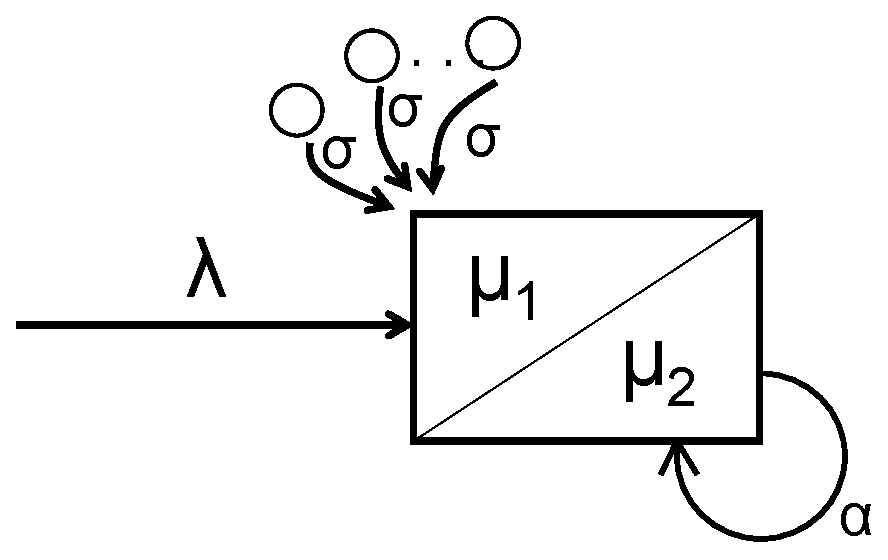
\includegraphics[scale=0.5]{common_model.eps}
	\caption{Общий вид RQ--системы с простейшим входящим потоком}
	\label{common_model_fig}
\end{figure}
Введем следующие обозначения: $i(t)$ --- число заявок на орбите в момент времени $t$, $k(t)$ --- состояние прибора: $0$ --- прибор свободен, $1$ --- прибор занят обслуживанием заявки входящего потока, $2$ --- прибор занят обслуживанием вызванной заявки. 
 
Поскольку целью исследования является характеристика работы выходящего потока системы, будет рассмотрено два варианта предложенной модели --- с суммарным и двумерным выходящими потоками.
\subsection{Суммарный выходящий поток RQ--системы} \label{section_simple_summary}
Суммарный выходящий поток RQ--системы подразумевает, что приходящие заявки и заявки, вызываемые прибором самостоятельно, являются однородными, посему результат работы системы рассматривается как совокупность обслуженных заявок входящего потока и вызванных. 
\begin{figure}[H]
	\centering
	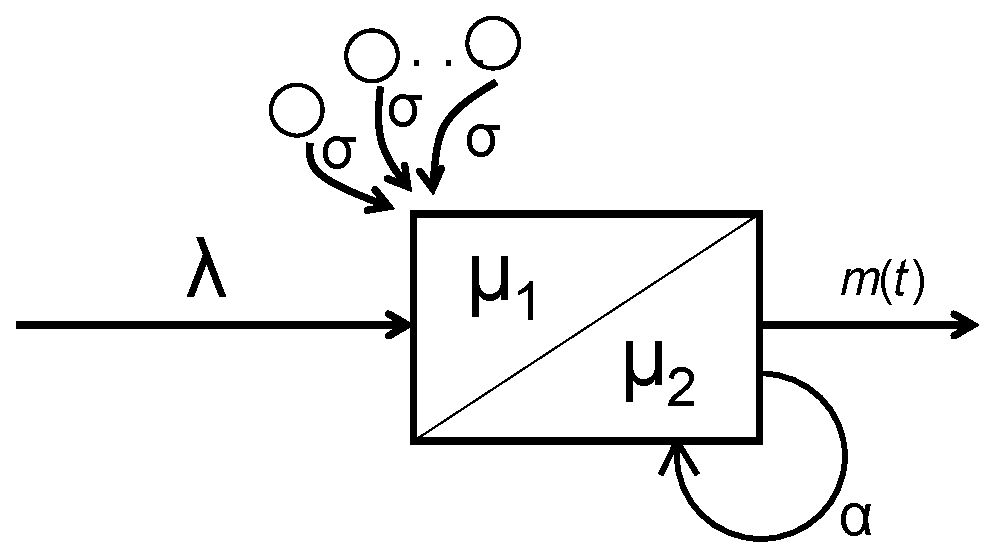
\includegraphics[scale=0.5]{summary_output_model.eps}
	\caption{Модель RQ--системы с суммарным выходящим потоком}
	\label{summary_output_model_fig}
\end{figure}
Введем обозначение: $m_(t)$ --- число обслуженных заявок в момент времени $t$.


\subsubsection{Уравнения Колмогорова}
Итак, мы имеем три характеристики, определяющие результат функционирования системы за некоторое время $t$: состояние прибора --- $k(t)$, количество заявок на орбите --- $i(t)$ и количество обслуженных заявок --- $m(t)$, что можно представить в виде трехмерного Марковского процесса
\begin{equation*}
	\{k(t),i(t),m(t)\}.
\end{equation*}

Заметим, что именно такая комбинация характеристик будет являться Марковским процессом, так как даёт достаточно информации о том, какое состояние система примет в следующий момент времени. Для этого необходимо знать, в каком состоянии прибор был в предшествующий момент времени, и какое количество заявок находилось в источнике повторных вызовов.
Следующее состояние, которое прибор может принять, зависит от состояния, в котором он находился прежде, то есть, каждое из трех состояний $k(t)$ принимается прибором с некоторыми вероятностями. Введем их в рассмотрение
\begin{equation*}
	\begin{split}
		P\{k(t)=0,i(t)=i,m(t)=m\} &=P_{0}(i,m,t),\\
		P\{k(t)=1,i(t)=i,m(t)=m\} &=P_{1}(i,m,t),\\
		P\{k(t)=2,i(t)=i,m(t)=m\} &=P_{2}(i,m,t).
	\end{split}
\end{equation*}

Теперь, необходимо определить вероятность перехода в каждое из трех состояний. Для этого обратимся к модели и рассмотрим $k(t) = 0$, то есть, состояние, в котором прибор свободен. Чтобы в следующий момент времени $t+\Delta t$ прибор был свободен необходимо выполнение одного из следующих условий:
\begin{enumerate}
	\item Прибор был свободным в момент времени $t$ и к моменту времени $t+\Delta t$  прибор не вызвал заявку, не пришла заявка с входящего потока и не было обращений заявок с орбиты.
	\item На момент времени $t+\Delta t$ прибор закончил обслуживание заявки с входящего потока.
	\item На момент времени $t+\Delta t$ прибор закончил обслуживание вызываемой заявки.
\end{enumerate}
Таким образом, применяя формулу полной вероятности, вероятность того, что прибор окажется свободен в момент времени $t+\Delta t$, равна сумме вероятностей наступления вышеперечисленных условий:
\begin{equation*}
	\begin{split}
	P_{0}(i,m,t+\Delta t) &=P_{0}(i,m,t)(1-\alpha\Delta t)(1 - i\sigma\Delta t)(1-\lambda\Delta t)+ \\ &+ P_{1}(i,m-1,t)\mu_{1}\Delta t + P_{2}(i,m-1,t)\mu_{2}\Delta t.
	\end{split}
\end{equation*}

Аналогично, для принятия состояния, в котором прибор занят, необходимо выполнение одного из следующих условий:
\begin{enumerate}
	\item Прибор был занят в момент времени $t$,  и к моменту времени $t+\Delta t$ прибор не закончил обслуживание заявки, и не пришла заявка с входящего потока.
	\item Прибор был свободен, и пришла заявка с входящего потока.
	\item Прибор был свободен, и повторно обратилась заявка с орбиты.
	\item Прибор был занят, и пришла заявка с входящего потока, сразу переместившись на орбиту.
\end{enumerate}
В результате получим следующее равенство:
\begin{equation*}
	\begin{split}
			P_{1}(i,m,t+\Delta t)&=P_{1}(i,m,t)(1-\lambda\Delta t)(1-\mu_{1}\lambda\Delta t)+P_{0}(i,m,t)\lambda\Delta t +\\ &+ P_{0}(i+1,m,t)(i+1)\sigma\Delta t + P_{1}(i-1,m,t)\lambda\Delta t + o(t).
	\end{split}
\end{equation*}

Вероятность принятия прибором состояния обслуживания вызываемой заявки является суммой следующих вероятностей:
\begin{enumerate}
	\item Прибор обслуживал вызываемую заявку и к моменту времени $t+\Delta t$ не закончил ее обслуживание, и не пришла заявка с входящего потока.
	\item Прибор обслуживал вызываемую заявку, и пришла заявка с входящего потока. Поскольку прибор занят, она ушла на орбиту.
	\item Прибор был свободен, и он вызвал заявку.
\end{enumerate}
Получим равенство:
\begin{equation*}
	\begin{split}
	P_{2}(i,m,t+\Delta t) &=P_{2}(i,m,t)(1-\alpha\Delta t)(1 - \lambda\Delta t)(1 - \mu_{2}\Delta t)+ \\ &+ P_{2}(i-1,m,t)\lambda\Delta t + P_{0}(i,m,t)\alpha\Delta t + o(t).
\end{split}
\end{equation*}

Запишем получившуюся систему уравнений
\begin{equation*} 
	\begin{split}
		P_{0}(i,m,t+\Delta t)&=P_{0}(i,m,t)(1-\alpha\Delta t)(1 - i\sigma\Delta t)(1-\lambda\Delta t) +\\ &+ P_{1}(i,m-1,t)\mu_{1}\Delta t + P_{2}(i,m-1,t)\mu_{2}\Delta t,
		\\
		P_{1}(i,m,t+\Delta t)&=P_{1}(i,m,t)(1-\lambda\Delta t)(1-\mu_{1}\lambda\Delta t)+P_{0}(i,m,t)\lambda\Delta t +\\ &+ P_{0}(i+1,m,t)(i+1)\sigma\Delta t + P_{1}(i-1,m,t)\lambda\Delta t + o(t),
		\\
		P_{2}(i,m,t+\Delta t)&=P_{2}(i,m,t)(1-\alpha\Delta t)(1 - \lambda\Delta t)(1 - \mu_{2}\Delta t) +\\ &+ P_{2}(i-1,m,t)\lambda\Delta t + P_{0}(i,m,t)\alpha\Delta t + o(t).
	\end{split}
\end{equation*}
Так как все слагаемые содержат $\Delta t$, разделим систему на $\Delta t$ и сделаем предельный переход $\Delta t \rightarrow 0$
\begin{equation} \label{kolmogorov_equations_summary}
	\begin{split}
		\frac{{\partial P_{0}(i,m,t)}}{{\partial t}} &= -(\lambda + i\sigma + \alpha)P_{0}(i,m,t) + P_{1}(i,m-1,t)\mu_{1} + P_{2}(i,m-1,t)\mu_{2},
		\\
		\frac{{\partial P_{1}(i,m,t)}}{{\partial t}} &= -(\lambda + \mu_{1})P_{1}(i,m,t) + (i+1)\sigma P_{0}(i+1,m,t) + \lambda  P_{0}(i,m,t),
		\\
		\frac{{\partial P_{2}(i,m,t)}}{{\partial t}} &= -(\lambda + \mu_{2})P_{2}(i,m,t) + \lambda P_{2}(i-1,m,t) + \alpha  P_{0}(i,m,t).
	\end{split}
\end{equation}	

Полученная система уравнений --- система дифференциальных уравнений Колмогорова, где в левой части каждого уравнения находится производная вероятности состояния рассматриваемого процесса, а в правой --- сумма произведений вероятностей состояний, из которых прибор может принять это состояние, на интенсивности соответствующих потоков заявок. Решением данной системы будут являться вероятности всех состояний прибора в виде функций времени. Таким образом, задача сводится к решению данной системы дифференциальных уравнений.

Решить данную систему аналитически не получится, так как это система бесконечного числа дифференциальных конечно--разностных уравнений с переменными коэффициентами. 
Для того, чтобы перейти к конечному числу уравнений, введем частные характеристические функции, обозначив $j=\sqrt{-1}$,
\begin{equation*}
	H_{k}(u_{1},u,t) = \sum_{i=0}^{\infty}
	\sum_{m=0}^{\infty}  
	e^{ju_{1}i}e^{jum} P_{k}(i,m,t).
\end{equation*}
Тогда перепишем систему \eqref{kolmogorov_equations_summary} в виде
\begin{equation} \label{characteristic_equations_summary}
	\begin{split}
		\frac{{\partial H_{0}(u_{1},u,t)}}{{\partial t}} &= -(\lambda + \alpha)H_{0}(u_{1},u,t) + j\sigma
		\frac{{\partial H_{0}(u_{1},u,t)}}{{\partial u_{1}}} +\\  &+ \mu_{1} e^{ju}H_{1}(u_{1},u,t) + \mu_{2}e^{ju}H_{2}(u_{1},u,t) ,
		\\
		\frac{{\partial H_{1}(u_{1},u,t)}}{{\partial t}} &= -(\lambda + \mu_{1})H_{1}(u_{1},u,t) - j\sigma e^{-ju_{1}}
		\frac{{\partial H_{0}(u_{1},u,t)}}{{\partial u_{1}}} +\\  &+ \lambda H_{0}(u_{1},u,t) + \lambda e^{ju_{1}}H_{1}(u_{1},u,t) ,
		\\
		\frac{{\partial H_{2}(u_{1},u,t)}}{{\partial t}} &= -(\lambda + \mu_{2})H_{2}(u_{1},u,t)  + \lambda e^{ju_{1}}H_{2}(u_{1},u,t) +\\  &+ \alpha H_{0}(u_{1},u,t).
	\end{split}
\end{equation}  

Таким образом, мы получили ровно три дифференциальных уравнения в частных производных с переменными коэффициентами.
\subsubsection{Метод асимптотического анализа}
Полученную систему дифференциальных уравнений в частных производных \eqref{characteristic_equations_summary} будем решать методом асимптотического анализа \cite{nazarov2017asymptotic} в предельном условии большой задержки заявок на орбите ($\sigma \rightarrow 0$).
Обозначим $\epsilon = \sigma,   u_{1}= \epsilon w,   F_{k}(w,u,t,\epsilon) = H_{k}(u_{1},u,t)$, тогда система запишется в виде
\begin{equation} \label{asymptotic_equations_summary}
	\begin{split}
		\frac{{\partial F_{0}(w,u,t,\epsilon)}}{{\partial t}} &= -(\lambda + \alpha)F_{0}(w,u,t,\epsilon) + j
		\frac{{\partial F_{0}(w,u,t,\epsilon)}}{{\partial w}} +\\  &+ \mu_{1} e^{ju}F_{1}(w,u,t,\epsilon) + \mu_{2}e^{ju}F_{2}(w,u,t,\epsilon) ,
		\\
		\frac{{\partial F_{1}(w,u,t,\epsilon)}}{{\partial t}} &= -(\lambda + \mu_{1})F_{1}(w,u,t,\epsilon) - j e^{-j\epsilon w}
		\frac{{\partial F_{0}(w,u,t,\epsilon)}}{{\partial w}} +\\  &+ \lambda F_{0}(w,u,t,\epsilon) + \lambda e^{j\epsilon w}F_{1}(w,u,t,\epsilon) ,
		\\
		\frac{{\partial F_{2}(w,u,t,\epsilon)}}{{\partial t}} &= -(\lambda + \mu_{2})F_{2}(w,u,t,\epsilon)  + \lambda e^{j\epsilon w}F_{2}(w,u,t,\epsilon) +\\  &+ \alpha F_{0}(w,u,t,\epsilon).
	\end{split}
\end{equation}  

С помощью введенных функций можно записать характеристическую функцию процесса $m(t)$ в следующем виде
\begin{equation*}
	M\{\exp(jum(t))\}=\sum_{k=0}^{2}H_{k}(0,u_{1},u_{2},t) = \sum_{k=0}^{2}F_{k}(0,u_{1},u_{2},t,\epsilon).
\end{equation*}

\begin{theorem}
	Асимптотические приближение характеристической функции числа обслуженных заявок за некоторое время $t$ имеет вид
	\begin{equation*} \label{theorem_summary}
		\begin{split}
			\lim_{\sigma \xrightarrow{} 0} M\{\exp(jum(t))\} &= \lim_{\epsilon \xrightarrow{} 0} \sum_{k=0}^{2}F_{k}(0,u,t,\epsilon) = \boldsymbol{R} \cdot \exp\{G(u)t\} \cdot \boldsymbol{E},
		\end{split}
	\end{equation*}
	где 
	\begin{equation*}
		\boldsymbol{G}(u)=\begin{bmatrix}
			-(\lambda + \alpha + \kappa) & \mu_{1}e^{ju} &  \mu_{2}e^{ju}\\
			\kappa+\lambda & -\mu_{1} & 0\\
			\alpha & 	0 &	-\mu_{2}
		\end{bmatrix}^{T},
	\end{equation*}
	вектор--строка $\boldsymbol{R}=\{R_{0},R_{1},R_{2}\}$ --- стационарное распределение вероятности состояния прибора
	\begin{equation*}
		\boldsymbol{R}=\left\{\frac{\mu_{2}(\mu_{1} - \lambda)}{\mu_{1}(\mu_{2} - \alpha)},\frac{\lambda}{\mu_{1}},\frac{\alpha(\mu_{1} - \lambda)}{\mu_{1}(\mu_{2} + \alpha)}\right\},
	\end{equation*}
	$\kappa$ --- нормированное среднее число заявок на орбите
	\begin{equation*}
		\kappa = \frac{\lambda(\lambda \mu_{2} + \alpha \mu_{1})}{\mu_{2}(\mu_{1} - \lambda)},
	\end{equation*}
	а $\boldsymbol{E}$ --- единичный вектор--столбец соответствующей размерности.
\end{theorem}
\begin{proof}
	Делая предельный переход $\epsilon\xrightarrow{} 0$  в полученной системе \eqref{asymptotic_equations_summary}, система уравнений будет записана в виде
	\begin{equation} \label{eps_limit_summary}
		\begin{split}
			\frac{{\partial F_{0}(w,u,t)}}{{\partial t}} &= -(\lambda + \alpha)F_{0}(w,u,t) + j
			\frac{{\partial F_{0}(w,u,t)}}{{\partial w}} +\\  &+ \mu_{1} e^{ju}F_{1}(w,u,t) + \mu_{2}e^{ju}F_{2}(w,u,t) ,
			\\
			\frac{{\partial F_{1}(w,u,t)}}{{\partial t}} &= -(\lambda + \mu_{1})F_{1}(w,u,t) - j 
			\frac{{\partial F_{0}(w,u,t)}}{{\partial w}} +\\  &+ \lambda F_{0}(w,u,t) + \lambda F_{1}(w,u,t),
			\\
			\frac{{\partial F_{2}(w,u,t)}}{{\partial t}} &= -(\lambda + \mu_{2})F_{2}(w,u,t)  + \lambda F_{2}(w,u,t) +\\  &+ \alpha F_{0}(w,u,t).
		\end{split}
	\end{equation}  

	Решение системы \eqref{eps_limit_summary} будет получено в следующей форме
	\begin{equation} \label{solution_form_summary}
		F_{k}(w,u,t) = \Phi(w)F_{k}(u,t).
	\end{equation}  
	$\Phi(w)$ --- асимптотическое приближение характеристической функции числа заявок на орбите при условии большой задержки на орбите.
	
	Подставив \eqref{solution_form_summary} в систему \eqref{eps_limit_summary} и разделив обе части уравнений на $\Phi(w)$, получим
	\begin{equation} \label{preresult_summary}
		\begin{split}
			\frac{{\partial F_{0}(u,t)}}{{\partial t}} &= -(\lambda + \alpha)F_{0}(u,t) + j
			\frac{\Phi'(w) }{\Phi(w)}F_{0}(u,t) +\\  &+ \mu_{1} e^{ju}F_{1}(u,t) + \mu_{2}e^{ju}F_{2}(u,t) ,
			\\
			\frac{{\partial F_{1}(u,t)}}{{\partial t}} &= -(\lambda + \mu_{1})F_{1}(u,t) - j 
			\frac{\Phi'(w) }{\Phi(w)}F_{0}(u,t) +\\  &+ \lambda F_{0}(u,t) + \lambda F_{1}(u,t) ,
			\\
			\frac{{\partial F_{2}(u,t)}}{{\partial t}} &= -(\lambda + \mu_{2})F_{2}(u,t)  + \lambda F_{2}(u,t) +\\  &+ \alpha F_{0}(u,t).
		\end{split}
	\end{equation} 
	Заметим, что $w$ содержится только в отношении $\frac{\Phi'(w) }{\Phi(w)}$, а остальные слагаемые и левые части уравнений не зависят от $w$. Это означает, что  $\Phi(w)$ имеет вид экспоненты. Учитывая, что  $\Phi(w)$ имеет смысл асимптотического приближения характеристической функции числа заявок на орбите, мы можем конкретизировать вид данной функции
	\begin{equation} \label{Phi_concrete}
		\frac{\Phi'(w) }{\Phi(w)} = \frac{e^{j\kappa w}j\kappa}{e^{j\kappa w}},
	\end{equation} 
	где $\kappa$ --- нормированное среднее число заявок на орбите, которое было получено в \cite{nazarov2017asymptotic} и имеет вид 
	\begin{equation*}
		\kappa = \frac{\lambda(\lambda \mu_{2} + \alpha \mu_{1})}{\mu_{2}(\mu_{1} - \lambda)}.
	\end{equation*}
	Исходя из этого, система \eqref{preresult_summary} примет следующий вид
	\begin{equation} \label{result_summary}
		\begin{split}
			\frac{{\partial F_{0}(u,t)}}{{\partial t}} &= -(\lambda + \alpha+ \kappa)F_{0}(u,t) + \mu_{1} e^{ju}F_{1}(u,t) + \mu_{2}e^{ju}F_{2}(u,t) ,
			\\
			\frac{{\partial F_{1}(u,t)}}{{\partial t}} &= (\lambda + \kappa)F_{0}(u,t) -  
			\mu_{1}F_{1}(u,t) +  0F_{2}(u,t) ,
			\\
			\frac{{\partial F_{2}(u,t)}}{{\partial t}} &= \alpha F_{0}(u,t)   +  0F_{1}(u,t) - \mu_{2}F_{2}(,t).
		\end{split}
	\end{equation}  

	Введем следующие обозначения
	\begin{equation*}
		\boldsymbol{F}(u,t) = \{F_{0}(u,t),F_{1}(u,t),F_{2}(u,t)\},
	\end{equation*}  
	\begin{equation*}
		\boldsymbol{G}(u)=\begin{bmatrix}
			-(\lambda + \alpha + \kappa) & \mu_{1}e^{ju} &  \mu_{2}e^{ju}\\
			\kappa+\lambda & -\mu_{1} & 0\\
			\alpha & 	0 &	-\mu_{2}
		\end{bmatrix}^{T},
	\end{equation*}
	$\boldsymbol{G}(u)$ --- транспонированная матрица коэффициентов системы \eqref{preresult_summary}.
	Тогда получим следующее матричное уравнение
	\begin{equation*}
		\frac{{\partial \boldsymbol{F}(u,t)}}{{\partial t}} =\boldsymbol{F}(u,t)\boldsymbol{G}(u),
	\end{equation*}
	общее решение которого имеет вид
	\begin{equation} \label{diff_summary}
		\boldsymbol{F}(u,t)=\boldsymbol{C}e^{\boldsymbol{G}(u)t}.
	\end{equation}

	Для того, чтобы получить единственное решение, которое соответствует поведению рассматриваемой системы, примем к рассмотрению начальное условие
	\begin{equation} \label{cauchi_condition_summary}
		\boldsymbol{F}(u,0)=\boldsymbol{R},
	\end{equation}
	где вектор--строка $\boldsymbol{R}$ --- стационарное распределение вероятности состояния прибора, то есть процесса $k(t)$, которое имеет форму \cite{nazarov2017asymptotic}
	\begin{equation*}
		\boldsymbol{R}=\left\{\frac{\mu_{2}(\mu_{1} - \lambda)}{\mu_{1}(\mu_{2} - \alpha)},\frac{\lambda}{\mu_{1}},\frac{\alpha(\mu_{1} - \lambda)}{\mu_{1}(\mu_{2} + \alpha)}\right\}.
	\end{equation*}

	Описав начальное условие, мы можем перейти к решению задачи Коши (\ref{diff_summary},\ref{cauchi_condition_summary}).
	Поскольку нас интересует распределение вероятностей количества заявок в выходном процессе, необходимо найти маргинальное распределение. Для этого суммируем компоненты вектор--строки $\boldsymbol{F}(u,t)$ по $k$ и умножаем результат на единичный вектор--столбец $\boldsymbol{E}$. Получим
	\begin{equation}\label{approximation_summary}
		\boldsymbol{F}(u,t)\boldsymbol{E}=\boldsymbol{R}e^{\boldsymbol{G}(u)t}\boldsymbol{E}.
	\end{equation}
	Эта формула позволяет найти асимптотическое приближение характеристической функции количества заявок, обслуженных системой к некоторому моменту времени $t$. Другими словами, формула \eqref{approximation_summary} является решением рассматриваемой системы. 
\end{proof}


\subsubsection{Переход к явному распределению вероятностей}
Полученная характеристическая функция \eqref{approximation_summary} так же, как и распределение вероятностей полностью описывает процесс $m(t)$, однако делает это в неявном виде. Поэтому для использования полученной формулы для вычислений необходимо получить из нее распределение вероятности.
Но прежде заметим, что в полученной формуле \eqref{approximation_summary} содержится матричная экспонента, вычислить которую в ее исходном виде не получится. Для преобразования экспоненты применим преобразование подобия \cite{bronson1991matrix}, которое выглядит следующим образом
\begin{equation*}
	\boldsymbol{G}(u) =\boldsymbol{T}(u)\boldsymbol{GJ}(u)\boldsymbol{T}(u)^{-1},
\end{equation*}
где $\boldsymbol{T}(u)$ – матрица собственных векторов матрицы $\boldsymbol{G}(u)$, а $\boldsymbol{GJ}(u)$ --- диагональная матрица, содержащая собственные числа матрицы $\boldsymbol{G}(u)$. Данное преобразование справедливо для любой степени $m$ некоторой матрицы $\boldsymbol{A}^{m}$, из чего следует, что оно так же справедливо для матричный экспоненты \cite{egorov2006prog}
\begin{equation*}
	e^{\boldsymbol{G}(u)t}=\boldsymbol{T}(u)\cdot \begin{bmatrix}
		e^{t \Lambda_{1}(u)} & 0 &  0\\
		0 & e^{t \Lambda_{2}(u)} & 0\\
		0 & 0 &	e^{t \Lambda_{3}(u)}
	\end{bmatrix} \cdot \boldsymbol{T}(u)^{-1},
\end{equation*}
где $\Lambda_{n}$ --- собственное число матрицы $\boldsymbol{G}(u)$. Тогда распределение примет следующий вид
\begin{equation*}
	\boldsymbol{F}(u,t)\boldsymbol{E}=\boldsymbol{R} \cdot \boldsymbol{T}(u)\cdot \begin{bmatrix}
		e^{t \Lambda_{1}(u)} & 0 &  0\\
		0 & e^{t \Lambda_{2}(u)} & 0\\
		0 & 0 &	e^{t \Lambda_{3}(u)}
	\end{bmatrix} \cdot \boldsymbol{T}(u)^{-1} \cdot \boldsymbol{E}.
\end{equation*}

Для того, чтобы получить явное распределение вероятностей числа обслуженных заявок, воспользуемся свойством характеристической функции, из которого следует, что распределение всегда восстанавливается по характеристической функции. Для обращения функции применим обратное преобразование Фурье для дискретных случайных величин
\begin{equation} \label{distr_simple_summary}
	P(m,t) = \dfrac{1}{2\pi}\int_{-\pi}^{\pi} e^{-i \cdot u \cdot m} \boldsymbol{F}(u,t)\boldsymbol{E}du.
\end{equation}

Полученное распределение характеризует вероятность обслуживания $m$ заявок к моменту времени $t$ в рассматриваемой системе.
\clearpage
\subsection{RQ-система с двумерным выходящим потоком}
В этом разделе будет рассмотрена модель RQ-системы, выходящий поток заявок которой, является двумерным. Другими словами, в системе обслуживаются два типа заявок - пришедшее извне и вызванные. Исходя из этого добавим к имеющимся обозначениям следующие: \textit{$m_{1}(t)$} — число обслуженных заявок входящего потока к моменту времени $\textit{t}$, \textit{$m_{2}(t)$} — обслуженных вызванных заявок к моменту времени $\textit{t}$.
\begin{figure}[H]
	\centering
	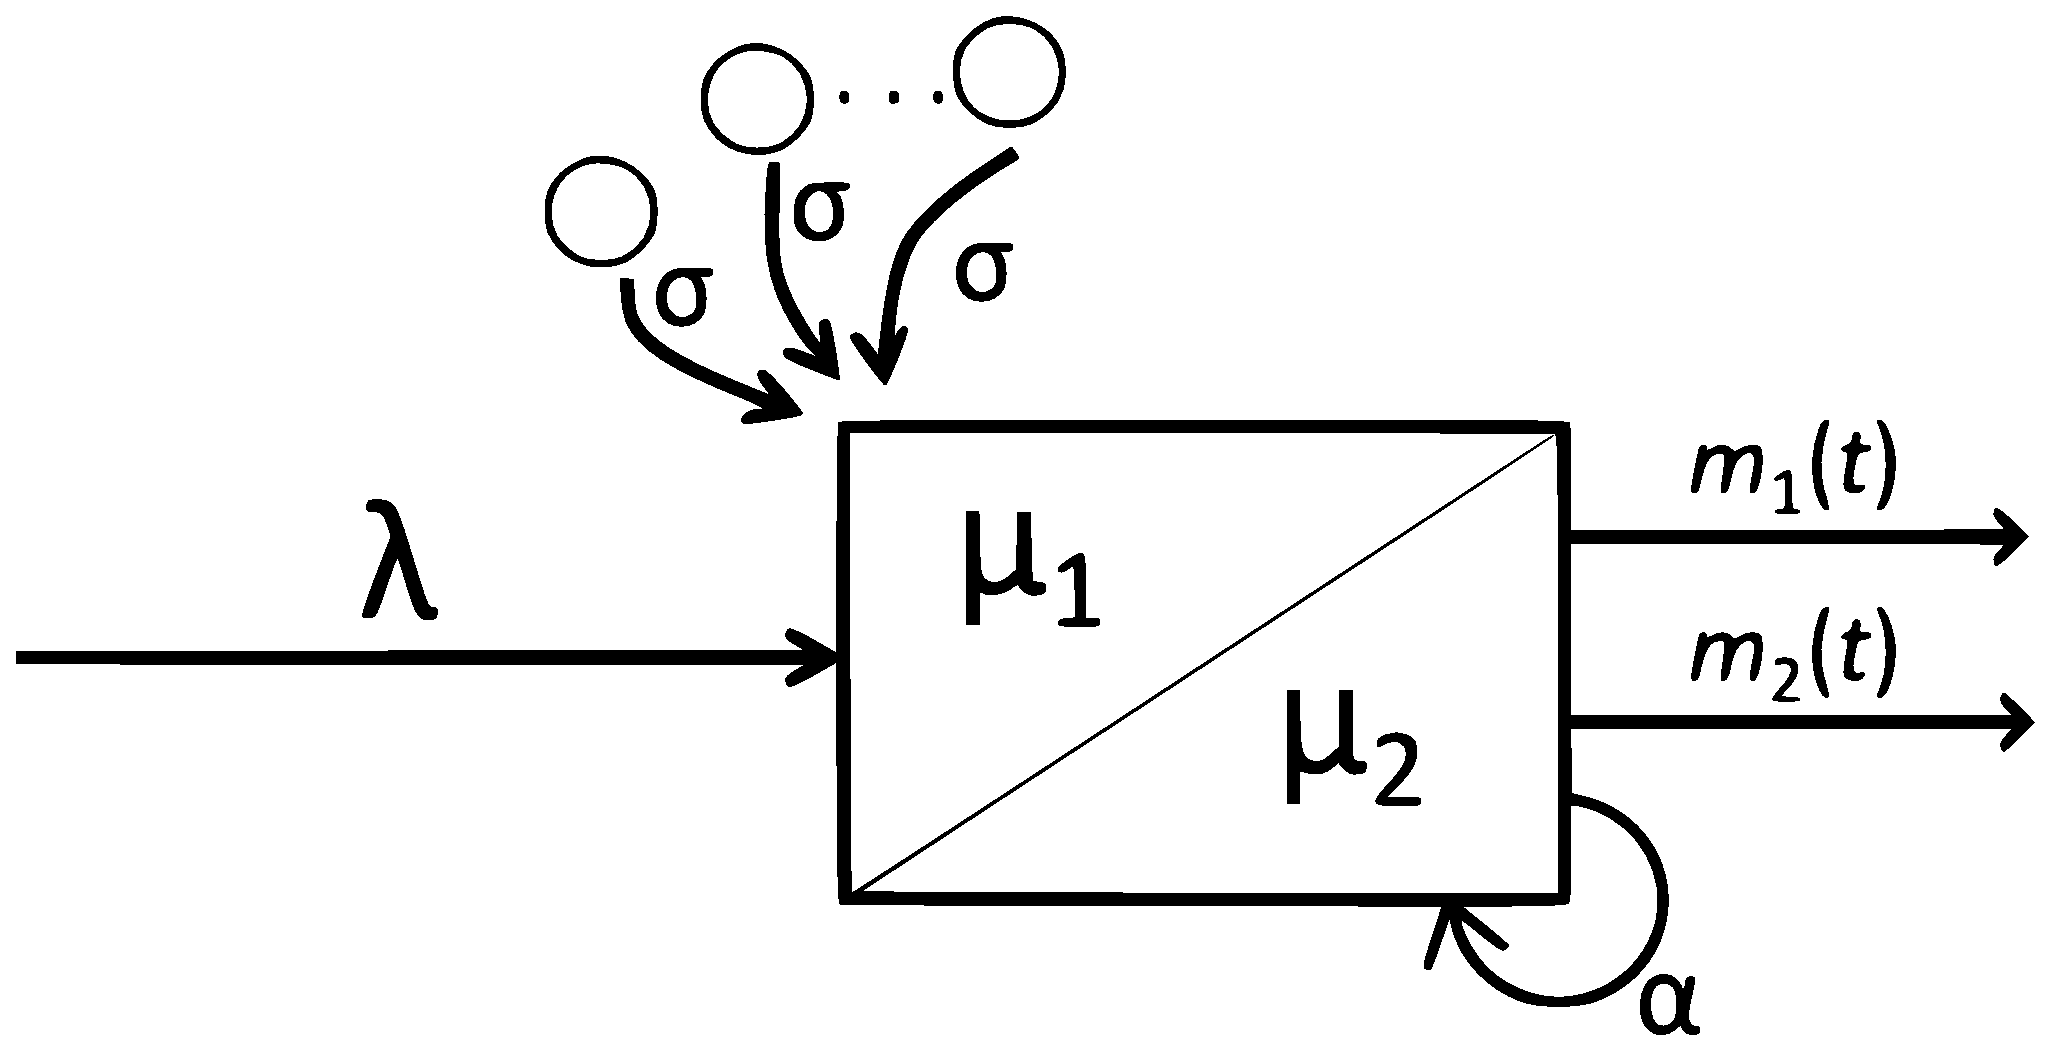
\includegraphics[scale=0.25]{twodim_output_model.eps}
	\caption{Модель RQ-системы с двумерным выходящим потоком}
	\label{twodim_output_model_fig}
\end{figure}
Функционирование данной системы аналогично рассмотренной ранее, посему процесс ее решения будет схож. 
\subsubsection{Уравнения Колмогорова}
В данном случае, мы имеем четыре характеристики, определяющие результат функционирования системы за некоторое время $\textit{i(t)}$: состояние прибора – $\textit{k(t)}$, количество заявок на орбите – $\textit{i(t)}$, количество обслуженных заявок входящего потока – $m_{1}(t)$, количество обслуженных вызванных заявок – $m_{2}(t)$,  что можно представить в виде четырех-мерного Марковского процесса
\begin{equation*}
	\{k(t),i(t),m_{1}(t),m_{2}(t)\}
\end{equation*}
Аналогично системе с суммарным выходящим потоком, следующее состояние зависит от предыдущего, вероятность принятия прибором одного из трех состояний задается, как
\begin{equation*}
	\begin{split}
		P\{k(t)=0,i(t)=i,m_{1}(t)=m_{1},m_{2}(t)=m_{2}\} &=P_{0}(i,m_{1},m_{2},t)\\
		P\{k(t)=1,i(t)=i,m_{1}(t)=m_{1},m_{2}(t)=m_{2}\} &=P_{1}(i,m_{1},m_{2},t)\\
		P\{k(t)=2,i(t)=i,m_{1}(t)=m_{1},m_{2}(t)=m_{2}\} &=P_{2}(i,m_{1},m_{2},t)
	\end{split}
\end{equation*}
Запишем систему уравнений Колмогорова, составленную на основе введенных вероятностей перехода
\begin{equation} \label{kolmogorov_equations_twodim}
	\begin{split}
		\frac{{\partial P_{0}(i,m_{1},m_{2},t)}}{{\partial t}} &= -(\lambda + i\sigma + \alpha)P_{0}(i,m_{1},m_{2},t) + P_{1}(i,m_{1}-1,m_{2},t)\mu_{1} +\\  &+ P_{2}(i,m_{1},m_{2}-1,t)\mu_{2} ,
		\\
		\frac{{\partial P_{1}(i,m_{1},m_{2},t)}}{{\partial t}} &= -(\lambda + \mu_{1})P_{1}(i,m_{1},m_{2},t) + (i+1)\sigma P_{0}(i+1,m_{1},m_{2},t) +\\ &+ \lambda  P_{0}(i,m_{1},m_{2},t),
		\\
		\frac{{\partial P_{2}(i,m_{1},m_{2},t)}}{{\partial t}} &= -(\lambda + \mu_{2})P_{2}(i,m_{1},m_{2},t) + \lambda P_{2}(i-1,m_{1},m_{2},t)  +\\ &+ \alpha  P_{0}(i,m_{1},m_{2},t).
	\end{split}
\end{equation}	
Введем частные характеристические функции, обозначив $j=\sqrt{-1}$,
\begin{equation*}
	H_{k}(u,u_{1},u_{2},t) = \sum_{i=0}^{\infty}
	\sum_{m_{1}=0}^{\infty}
	\sum_{m_{2}=0}^{\infty}  
	e^{jui}e^{ju_{1}m_{1}}e^{ju_{2}m_{2}} P_{k}(i,m_{1},m_{2},t).
\end{equation*}
Тогда перепишем систему (\ref{kolmogorov_equations_twodim}) в виде
\begin{equation} \label{characteristic_equations_twodim}
	\begin{split}
		\frac{{\partial H_{0}(u,u_{1},u_{2},t)}}{{\partial t}} &= -(\lambda + \alpha)H_{0}(u,u_{1},u_{2},t) + j\sigma
		\frac{{\partial H_{0}(u,u_{1},u_{2},t)}}{{\partial u}} +\\  &+ \mu_{1} e^{ju_{1}}H_{1}(u,u_{1},u_{2},t) + \mu_{2}e^{ju_{2}}H_{2}(u,u_{1},u_{2},t) ,
		\\
		\frac{{\partial H_{1}(u,u_{1},u_{2},t)}}{{\partial t}} &= -(\lambda + \mu_{1})H_{1}(u,u_{1},u_{2},t) - j\sigma e^{-ju}
		\frac{{\partial H_{0}(u,u_{1},u_{2},t)}}{{\partial u}} +\\  &+ \lambda H_{0}(u,u_{1},u_{2},t) + \lambda e^{ju}H_{1}(u,u_{1},u_{2},t) ,
		\\
		\frac{{\partial H_{2}(u,u_{1},u_{2},t)}}{{\partial t}} &= -(\lambda + \mu_{2})H_{2}(u,u_{1},u_{2},t)  + \lambda e^{ju}H_{2}(u,u_{1},u_{2},t) +\\  &+ \alpha H_{0}(u,u_{1},u_{2},t).
	\end{split}
\end{equation}  
Бесконечное количество уравнений сведено к трем.

\subsubsection{Метод асимптотического анализа}
Полученную систему дифференциальных уравнений в частичных производных  (\ref{characteristic_equations_twodim}) будем решать методом асимптотического анализа в предельном условии большой задержки заявок на орбите ($\sigma \xrightarrow{} 0$).

Обозначим $\epsilon = \sigma,   u= \epsilon w,   F_{k}(w,u_{1},u_{2},t,\epsilon) = H_{k}(u,u_{1},u_{2},t)$, тогда система запишется в виде
\begin{equation} \label{asymptotic_equations_twodim}
	\begin{split}
		\frac{{\partial F_{0}(w,u_{1},u_{2},t,\epsilon)}}{{\partial t}} &= -(\lambda + \alpha)F_{0}(w,u_{1},u_{2},t,\epsilon) + j
		\frac{{\partial F_{0}(w,u_{1},u_{2},t,\epsilon)}}{{\partial w}} +\\  &+ \mu_{1} e^{ju_{1}}F_{1}(w,u_{1},u_{2},t,\epsilon) + \mu_{2}e^{ju_{2}}F_{2}(u,u_{1},u_{2},t,\epsilon) ,
		\\
		\frac{{\partial F_{1}(w,u_{1},u_{2},t,\epsilon)}}{{\partial t}} &= -(\lambda + \mu_{1})F_{1}(w,u_{1},u_{2},t,\epsilon) - j e^{-j\epsilon w}
		\frac{{\partial F_{0}(w,u_{1},u_{2},t,\epsilon)}}{{\partial w}} +\\  &+ \lambda F_{0}(w,u_{1},u_{2},t,\epsilon) + \lambda e^{j\epsilon w}F_{1}(w,u_{1},u_{2},t,\epsilon) ,
		\\
		\frac{{\partial F_{2}(w,u_{1},u_{2},t,\epsilon)}}{{\partial t}} &= -(\lambda + \mu_{2})F_{2}(w,u_{1},u_{2},t,\epsilon)  + \lambda e^{j\epsilon w}F_{2}(w,u_{1},u_{2},t,\epsilon) +\\  &+ \alpha F_{0}(w,u_{1},u_{2},t,\epsilon).
	\end{split}
\end{equation}  
Затем, что используя условие согласованности многомерных распределений, характеристическая функция процессов $m_{1}(t$) и $m_{1}(t)$ будет записана в следующем виде с введенными функциями 
\begin{equation*}
	M\{\exp(ju_{1}m_{1}(t))\exp(ju_{2}m_{2}(t))\}=\sum_{k=0}^{2}H_{k}(0,u_{1},u_{2},t) = \sum_{k=0}^{2}F_{k}(0,u_{1},u_{2},t,\epsilon).
\end{equation*}

\begin{theorem}
	Асимптотические приближение двумерной характеристической функции числа обслуженных заявок входящего потока и числа обслуженных вызванных заявок за некоторое время $t$ имеет вид
	\begin{equation*} \label{theorem_twodim}
		\begin{split}
			\boldsymbol{F}(u_{1},u_{2},t) =  \lim_{\sigma \xrightarrow{} 0} M\{\exp(ju_{1}m_{1}(t))\exp(ju_{2}m_{2}(t))\} &= 
			\\
			= \lim_{\epsilon \xrightarrow{} 0} \sum_{k=0}^{2}F_{k}(0,u_{1},u_{2},t,\epsilon) = \boldsymbol{R} \cdot \exp\{G(u_{1},u_{2})t\} \cdot \boldsymbol{E}
		\end{split}
	\end{equation*}
	где 
	\begin{equation*}
		\boldsymbol{G}(u_{1},u_{2})=\begin{bmatrix}
			-(\lambda + \alpha + \kappa) & \mu_{1}e^{ju_{1}} &  \mu_{2}e^{ju_{2}}\\
			\kappa+\lambda & -\mu_{1} & 0\\
			\alpha & 	0 &	-\mu_{2}
		\end{bmatrix}^{T},
	\end{equation*}
	вектор-строка $\boldsymbol{R}=\{R_{0},R_{1},R_{2}\}$ - стационарное распределение вероятности состояния прибора
	\begin{equation*}
		\boldsymbol{R}=\{\frac{\mu_{2}(\mu_{1} - \lambda)}{\mu_{1}(\mu_{2} - \alpha)},\frac{\lambda}{\mu_{1}},\frac{\alpha(\mu_{1} - \lambda)}{\mu_{1}(\mu_{2} + \alpha)}\},
	\end{equation*}
	$\kappa$ - нормированное среднее число заявок на орбите
	\begin{equation*}
		\kappa = \frac{\lambda(\lambda \mu_{2} + \alpha \mu_{1})}{\mu_{2}(\mu_{1} - \lambda)},
	\end{equation*}
	а $\boldsymbol{E}$ - единичный вектор-столбец соответствующей размерности.
\end{theorem}
\begin{proof}
	Делая предельный переход $ \lim_{\epsilon \xrightarrow{} 0} F_{k}(w,u_{1},u_{2},t,\epsilon) = F_{k}(w,u_{1},u_{2},t)$  в полученной системе (\ref{asymptotic_equations_twodim}) , система уравнений будет записана в виде
	\begin{equation} \label{eps_limit_twodim}
		\begin{split}
			\frac{{\partial F_{0}(w,u_{1},u_{2},t)}}{{\partial t}} &= -(\lambda + \alpha)F_{0}(w,u_{1},u_{2},t) + j
			\frac{{\partial F_{0}(w,u_{1},u_{2},t)}}{{\partial w}} +\\  &+ \mu_{1} e^{ju_{1}}F_{1}(w,u_{1},u_{2},t) + \mu_{2}e^{ju_{2}}F_{2}(w,u_{1},u_{2},t) ,
			\\
			\frac{{\partial F_{1}(w,u_{1},u_{2},t)}}{{\partial t}} &= -(\lambda + \mu_{1})F_{1}(w,u_{1},u_{2},t) - j 
			\frac{{\partial F_{0}(w,u_{1},u_{2},t)}}{{\partial w}} +\\  &+ \lambda F_{0}(w,u_{1},u_{2},t) + \lambda F_{1}(w,u_{1},u_{2},t) ,
			\\
			\frac{{\partial F_{2}(w,u_{1},u_{2},t)}}{{\partial t}} &= -(\lambda + \mu_{2})F_{2}(w,u_{1},u_{2},t)  + \lambda F_{2}(w,u_{1},u_{2},t) +\\  &+ \alpha F_{0}(w,u_{1},u_{2},t).
		\end{split}
	\end{equation}  
	Решение системы (\ref{eps_limit_twodim}) будет получено в следующей форме
	\begin{equation} \label{solution_twodim}
		F_{k}(w,u_{1},u_{2},t) = \Phi(w)F_{k}(u_{1},u_{2},t).
	\end{equation}  
	$\Phi(w)$ - асимптотическое приближение характеристической функции числа заявок на орбите при условии большой задержки на орбите.
	
	Подставив (\ref{solution_twodim}) в систему (\ref{eps_limit_twodim}) и разделив обе части уравнений на $\Phi(w)$, получим
	\begin{equation} \label{preresult_twodim}
		\begin{split}
			\frac{{\partial F_{0}(u_{1},u_{2},t)}}{{\partial t}} &= -(\lambda + \alpha)F_{0}(u_{1},u_{2},t) + j
			\frac{\Phi'(w) }{\Phi(w)}F_{0}(u_{1},u_{2},t) +\\  &+ \mu_{1} e^{ju_{1}}F_{1}(u_{1},u_{2},t) + \mu_{2}e^{ju_{2}}F_{2}(u_{1},u_{2},t) ,
			\\
			\frac{{\partial F_{1}(u_{1},u_{2},t)}}{{\partial t}} &= -(\lambda + \mu_{1})F_{1}(u_{1},u_{2},t) - j 
			\frac{\Phi'(w) }{\Phi(w)}F_{0}(u_{1},u_{2},t) +\\  &+ \lambda F_{0}(u_{1},u_{2},t) + \lambda F_{1}(u_{1},u_{2},t) ,
			\\
			\frac{{\partial F_{2}(u_{1},u_{2},t)}}{{\partial t}} &= -(\lambda + \mu_{2})F_{2}(u_{1},u_{2},t)  + \lambda F_{2}(u_{1},u_{2},t) +\\  &+ \alpha F_{0}(u_{1},u_{2},t).
		\end{split}
	\end{equation}  
	%Заметим, что $w$ содержится только в отношении $\frac{\Phi'(w) }{\Phi(w)}$, а остальные слагаемые и левые части уравнений не зависят от $w$. Это означает, что  $\Phi(w)$ имеет вид экспоненты. Учитывая, что  $\Phi(w)$ имеет смысл асимптотического приближения характеристической функции числа заявок на орбите, мы можем конкретизировать вид данной функции
	%\begin{equation*}
	%	\frac{\Phi'(w) }{\Phi(w)} = \frac{e^{j\kappa w}j\kappa}{e^{j\kappa w}},
	%\end{equation*} 
	%где $\kappa$ - нормированное среднее число заявок на орбите, которое было получено в %\cite{nazarov2017asymptotic} и имеет вид 
	%\begin{equation*}
%		\kappa = \frac{\lambda(\lambda \mu_{2} + \alpha \mu_{1})}{\mu_{2}(\mu_{1} - \lambda)}.
%	\end{equation*}
	Ранее, мы конкретизировали вид $\Phi(w)$ в (\ref{Phi_concrete}), что позволяет нам привести систему (\ref{preresult_twodim}) к следующему виду	
	\begin{equation} \label{result_twodim}
		\begin{split}
			\frac{{\partial F_{0}(u_{1},u_{2},t)}}{{\partial t}} &= -(\lambda + \alpha+ \kappa)F_{0}(u_{1},u_{2},t) + \\  &+ \mu_{1} e^{ju_{1}}F_{1}(u_{1},u_{2},t) + \mu_{2}e^{ju_{2}}F_{2}(u_{1},u_{2},t) ,
			\\
			\frac{{\partial F_{1}(u_{1},u_{2},t)}}{{\partial t}} &= (\lambda + \kappa)F_{0}(u_{1},u_{2},t) -  
			\mu_{1}F_{1}(u_{1},u_{2},t) +\\  &+  0F_{2}(u_{1},u_{2},t) ,
			\\
			\frac{{\partial F_{2}(u_{1},u_{2},t)}}{{\partial t}} &= \alpha F_{0}(u_{1},u_{2},t)   +  0F_{1}(u_{1},u_{2},t) -\\  &- \mu_{2}F_{2}(u_{1},u_{2},t).
		\end{split}
	\end{equation}  
	Введем следующие обозначения
	\begin{equation*}
		\boldsymbol{F}(u_{1},u_{2},t) = \{F_{0}(u_{1},u_{2},t),F_{1}(u_{1},u_{2},t),F_{1}(u_{2},u_{2},t)\},
	\end{equation*}  
	\begin{equation*}
		\boldsymbol{G}(u_{1},u_{2})=\begin{bmatrix}
			-(\lambda + \alpha + \kappa) & \mu_{1}e^{ju_{1}} &  \mu_{2}e^{ju_{2}}\\
			\kappa+\lambda & -\mu_{1} & 0\\
			\alpha & 	0 &	-\mu_{2}
		\end{bmatrix}^{T},
	\end{equation*}
	$\boldsymbol{G}(u_{1},u_{2})$ - транспонированная матрица коэффициентов системы (\ref{result_twodim}).
	Тогда получим следующее матричное уравнение
	\begin{equation*}
		\frac{{\partial \boldsymbol{F}(u_{1},u_{2},t)}}{{\partial t}} =\boldsymbol{F}(u_{1},u_{2},t)\boldsymbol{G}(u_{1},u_{2}),
	\end{equation*}
	общее решение которого имеет вид
	\begin{equation} \label{diff_twodim}
		\boldsymbol{F}(u_{1},u_{2},t)=\boldsymbol{C}e^{\boldsymbol{G}(u_{1},u_{2})t}.
	\end{equation}
	Для получения единственного решения примем в рассмотрение начальное условие
	\begin{equation} \label{cauchi_condition_twodim}
		\boldsymbol{F}(u_{1},u_{2},0)=\boldsymbol{R},
	\end{equation}
	где вектор-строка $\boldsymbol{R}$ - стационарное распределение вероятности состояния прибора, то есть процесса $k(t)$, которое имеет форму \cite{nazarov2017asymptotic}
	\begin{equation*}
		\boldsymbol{R}=\{\frac{\mu_{2}(\mu_{1} - \lambda)}{\mu_{1}(\mu_{2} - \alpha)},\frac{\lambda}{\mu_{1}},\frac{\alpha(\mu_{1} - \lambda)}{\mu_{1}(\mu_{2} + \alpha)}\}.
	\end{equation*}
	Описав начальное условие, переходим к решению задачи Коши (\ref{diff_twodim}, \ref{cauchi_condition_twodim}).
	
	Чтобы получить маргинальное распределение вероятностей числа обслуженных заявок, суммируем компоненты вектор-строки $\boldsymbol{F}(u_{1},u_{2},t)$ по $k$ и умножаем результат на единичный вектор-столбец $\boldsymbol{E}$. Получим
	\begin{equation}\label{approximation_twodim}
		\boldsymbol{F}(u_{1},u_{2},t)\boldsymbol{E}=\boldsymbol{R}e^{\boldsymbol{G}(u_{1},u_{2})t}\boldsymbol{E}.
	\end{equation}
	Формула (\ref{approximation_twodim}) является решением рассматриваемой системы. 
\end{proof}

\subsubsection{Переход к явному распределению вероятности} \label{distr_find_twodim}
Характеристическая функция (\ref{approximation_twodim}) описывает процессы $m_{1}(t)$ и $m_{2}(t)$, однако делает это в неявной форме. Для использования полученной формулы для расчетов, получим явное распределение вероятности.
Формула (\ref{approximation_twodim}), так же как и (\ref{approximation_summary}) содержит матричную экспоненту, к которой мы применим преобразование подобия \cite{bronson1991matrix}
\begin{equation*}
	\boldsymbol{G}(u_{1},u_{2}) =\boldsymbol{T}(u_{1},u_{2})\boldsymbol{GJ}(u_{1},u_{2})\boldsymbol{T}(u_{1},u_{2})^{-1},
\end{equation*}
где $\boldsymbol{T}(u_{1},u_{2})$ – матрицы собственных вектором матрицы $\boldsymbol{G}(u_{1},u_{2})$, а $\boldsymbol{GJ}(u_{1},u_{2})$ - диагональная матрицы, содержащая собственные числа $\boldsymbol{G}(u_{1},u_{2})$. Данное преобразование справедливо для любой степени $m$ некоторой матрицы $\boldsymbol{A}^{m}$, из чего следует, что оно так же справедливо для матричной экспоненты \ref{egorov2006prog}
\begin{equation*}
	e^{\boldsymbol{G}(u_{1},u_{2})t}=\boldsymbol{T}(u_{1},u_{2})\cdot \begin{bmatrix}
		e^{t \Lambda_{1}(u_{1},u_{2})} & 0 &  0\\
		0 & e^{t \Lambda_{2}(u_{1},u_{2})} & 0\\
		0 & 0 &	e^{t \Lambda_{3}(u_{1},u_{2})}
	\end{bmatrix} \cdot \boldsymbol{T}(u_{1},u_{2})^{-1},
\end{equation*}
где $\Lambda_{n}$ - собственное число матрицы $\boldsymbol{G}(u_{1},u_{2})$. Тогда распределение примет следующий вид
\begin{equation*}
	\boldsymbol{F}(u_{1},u_{2},t)=\boldsymbol{R} \cdot \boldsymbol{T}(u_{1},u_{2})\cdot \begin{bmatrix}
		e^{t \Lambda_{1}(u_{1},u_{2})} & 0 &  0\\
		0 & e^{t \Lambda_{2}(u_{1},u_{2})} & 0\\
		0 & 0 &	e^{t \Lambda_{3}(u_{1},u_{2})}
	\end{bmatrix} \cdot \boldsymbol{T}(u_{1},u_{2})^{-1} \cdot \boldsymbol{E}.
\end{equation*}
Для восстановления распределения используем обратное преобразование Фурье для дискретных величин
\begin{equation*}
	P(m_{1},m_{2},t) = \dfrac{1}{2\pi}\int_{-\pi}^{\pi}\int_{-\pi}^{\pi} e^{-i \cdot u_{1} \cdot m_{1}} e^{-i \cdot u_{2} \cdot m_{2}}\boldsymbol{F}(u_{1},u_{2},t)du_{2}du_{2}.
\end{equation*}
Полученная формула характеризует вероятность обслуживания $m_{1}$ входящих заявок и $m_{2}$ вызванных заявок к моменту времени $t$ в рассматриваемой системе.

\subsubsection{Коэффициент корреляции}
Полученное асимптотические приближение характеристической функции (\ref{approximation_twodim}) позволяет нам подробнее изучить выходящие потоки рассматриваемой системы, а именно – найти корреляционную зависимость случайных процессов $m_{1}(t)$ и $m_{2}(t)$.
Рассмотрим нахождение коэффициента корреляции, который будет зависеть от параметра $t$
\begin{equation*}
	r(t) = \frac{\textnormal{cov}(m_{1}(t),m_{2}(t))}{\sqrt{D(m_{1}(t))}\sqrt{D(m_{2}(t))}}.
\end{equation*}
Воспользуемся свойством характеристической функции о существовании ее $n$-ой производной, соответствующей $n$-му начальному моменту случайной величины. Тогда ковариация и дисперсия будут вычисляться следующим образом
\begin{equation*}
	\begin{split}
		\textnormal{cov}(m_{1}(t),m_{2}(t)) &= M\{m_{1}(t)m_{2}(t)\} - M\{m_{1}(t)\}M\{m_{2}(t)\} = \frac{1}{j^{2}}\frac{{\partial}^{2}}{{\partial u_{1}}{\partial u_{2}}}\boldsymbol{F}(u_{1},u_{2},t) \bigg\rvert_{\substack{u_{1} = 0 \\ u_{2} = 0}} - \\ &- \frac{1}{j^{2}} \frac{{\partial}}{{\partial u_{1}}} \boldsymbol{F}(u_{1},u_{2},t) \bigg\rvert_{\substack{u_{1} = 0 \\ u_{2} = 0}} \frac{{\partial}}{{\partial u_{2}}} \boldsymbol{F}(u_{1},u_{2},t) \bigg\rvert_{\substack{u_{1} = 0 \\ u_{2} = 0}},
		\\
		D\{m_{1}(t)\} &= M^{2}\{m_{1}(t)\} - (M\{m_{1}(t)\})^{2} = \frac{1}{j^{2}}\frac{{\partial}^{2}}{{\partial u_{1}}^{2}}\boldsymbol{F}(u_{1},u_{2},t) \bigg\rvert_{\substack{u_{1} = 0 \\ u_{2} = 0}}  - \\ &- (\frac{1}{j^{2}} \frac{{\partial}}{{\partial u_{1}}} \boldsymbol{F}(u_{1},u_{2},t) \bigg\rvert_{\substack{u_{1} = 0 \\ u_{2} = 0}})^{2},
		\\
		D\{m_{2}(t)\} &= M^{2}\{m_{2}(t)\} - (M\{m_{2}(t)\})^{2} = \frac{1}{j^{2}}\frac{{\partial}^{2}}{{\partial u_{2}}^{2}}\boldsymbol{F}(u_{1},u_{2},t) \bigg\rvert_{\substack{u_{1} = 0 \\ u_{2} = 0}}  - \\ &- (\frac{1}{j^{2}} \frac{{\partial}}{{\partial u_{2}}} \boldsymbol{F}(u_{1},u_{2},t) \bigg\rvert_{\substack{u_{1} = 0 \\ u_{2} = 0}})^{2}.
	\end{split}
\end{equation*}
Полученные формулы позволяют использовать нам численно исследовать поведение системы при разных параметрах.
\clearpage
 %Простейший поток
\section {\centering Исследование систем с MMPP--потоком} \label{mmpp_section}
В этом разделе предлагается к рассмотрению система обслуживания, в которой в качестве источника входящих заявок выступает MMPP--поток.

MMPP (Markov Modulated Poisson Process) представляет собой поток заявок, управляемый непрерывной цепью Маркова. Изменение состояния влечет за собой изменение интенсивности прихода заявок. Данный тип входящего потока широко используется для моделирования телекоммуникационных сетей, поскольку он точно описывает изменяющуюся во времени скорость поступления заявок и фиксирует некоторые важные корреляции между временами прибытия, оставаясь при этом поддающимся анализу \cite{fischer1993markov}.
 
Для того, чтобы описать изменение состояние MMPP--потока во времени используются две матрицы.

Матрица инфинитезимальных характеристик $Q$. Величина $q_{ij}$ определяет интенсивность перехода процесса из $i$--ого в $j$--ое состояние, а величина $-q_{ii}$ --- интенсивность выхода из состояния $i$.
Матрица $Q$ имеет свойство $\sum_{j}q_{ij} = 0$
\begin{equation*}
	\boldsymbol{Q}=\begin{bmatrix}
		q_{11} &  \dots &  q_{1n}\\
		\vdots & \ddots &  \\
		q_{n1} &    	&	q_{nn}
	\end{bmatrix}
\end{equation*}
Диагональная матрица $\Lambda$ задаёт интенсивность поступления заявок для каждого из состояний процесса.
\begin{equation*}
	\boldsymbol{\Lambda}=\begin{bmatrix}
		\lambda_{11}&	\dots	&   	 & 0\\
		\vdots 		&\lambda_{22}&  	 &   \\
		       		&    		& \ddots &   \\
		0  			&   \dots 	&		 & \lambda_{nn}
	\end{bmatrix}
\end{equation*}

\subsection{Двумерный выходящий поток RQ--системы с MMPP} \label{section_map_twodim}
В случае RQ--системы с MMPP--потоком, к описанной ранее общей модели добавляется так же процесс $n_(t)$ --- состояние входящего потока в момент времени $t$. Тогда, результат функционирования системы будет описываться пяти--мерным Марковским процессом
\begin{equation*}
	\{k(t),n(t),i(t),m_{1}(t),m_{2}(t)\}.
\end{equation*}

\subsubsection{Уравнения Колмогорова}
Исходя из описанного Марковского процесса, вероятности того, что прибор будет находится в одном из трех состояний $k$, на орбите будет $i$ заявок, $m_{1}$ заявок входящего потока и $m_{2}$ вызванных заявок будет обслужено, а управляющая MMPP--потоком цепь Маркова будет находится в состоянии $n$ будут иметь вид
\begin{equation*}
	\begin{split}
		P\{k(t)=0,n(t)=n,i(t)=i,m_{1}(t)=m_{1},m_{2}(t)=m_{2}\} &=P_{0}(n,i,m_{1},m_{2},t),\\
		P\{k(t)=1,n(t)=n,i(t)=i,m_{1}(t)=m_{1},m_{2}(t)=m_{2}\} &=P_{1}(n,i,m_{1},m_{2},t),\\
		P\{k(t)=2,n(t)=n,i(t)=i,m_{1}(t)=m_{1},m_{2}(t)=m_{2}\} &=P_{2}(n,i,m_{1},m_{2},t).
	\end{split}
\end{equation*} 

На основе данных вероятностей запишем систему уравнений Колмогорова с учетом текущего состояния входящего потока
\begin{equation} \label{kolmogorov_equations_twodim_map}
	\begin{split}
		\frac{{\partial P_{0}(n,i,m_{1},m_{2},t)}}{{\partial t}} &= -(\lambda_{n} + i\sigma + \alpha)P_{0}(n,i,m_{1},m_{2},t) + P_{1}(n,i,m_{1}-1,m_{2},t)\mu_{1} +\\  &+ P_{2}(n,i,m_{1},m_{2}-1,t)\mu_{2} + \sum_{v=1}^{N} P_{0}(v,i,m_{1},m_{2},t)q_{vn},
		\\
		\frac{{\partial P_{1}(n,i,m_{1},m_{2},t)}}{{\partial t}} &= -(\lambda_{n} + \mu_{1})P_{1}(n,i,m_{1},m_{2},t) + (i+1)\sigma P_{0}(n,i+1,m_{1},m_{2},t) +\\ &+ \lambda_{n}  P_{0}(i,m_{1},m_{2},t) + \sum_{v=1}^{N}P_{1}(v,i,m_{1},m_{2},t)q_{vn},
		\\
		\frac{{\partial P_{2}(n,i,m_{1},m_{2},t)}}{{\partial t}} &= -(\lambda_{n} + \mu_{2})P_{2}(n,i,m_{1},m_{2},t) + \lambda_{n} P_{2}(n,i-1,m_{1},m_{2},t)  +\\ &+ \alpha  P_{0}(n,i,m_{1},m_{2},t) +  \sum_{v=1}^{N}P_{2}(v,i,m_{1},m_{2},t)q_{vn}.
	\end{split}
\end{equation}	

Введем частные характеристические функции, обозначив $j=\sqrt{-1}$
\begin{equation*}
	H_{k}(n,u,u_{1},u_{2},t) = \sum_{i=0}^{\infty}
	\sum_{m_{1}=0}^{\infty}
	\sum_{m_{2}=0}^{\infty}  
	e^{jui}e^{ju_{1}m_{1}}e^{ju_{2}m_{2}} P_{k}(n,i,m_{1},m_{2},t).
\end{equation*}
Перепишем систему \eqref{kolmogorov_equations_twodim_map} с учетом введенных частных характеристических функций
\begin{equation} \label{characteristic_equations_twodim_map}
	\begin{split}
		\frac{{\partial H_{0}(n,u,u_{1},u_{2},t)}}{{\partial t}} &= -(\lambda_{n} + \alpha)H_{0}(n,u,u_{1},u_{2},t) + j\sigma
		\frac{{\partial H_{0}(n,u,u_{1},u_{2},t)}}{{\partial u}} +\\  &+ \mu_{1} e^{ju_{1}}H_{1}(n,u,u_{1},u_{2},t) + \mu_{2}e^{ju_{2}}H_{2}(n,u,u_{1},u_{2},t) +\\  &+ \sum_{v=1}^{N}H_{0}(v,u,u_{1},u_{2},t)q_{vn} ,
		\\
		\frac{{\partial H_{1}(n,u,u_{1},u_{2},t)}}{{\partial t}} &= -(\lambda_{n} + \mu_{1})H_{1}(n,u,u_{1},u_{2},t) - j\sigma e^{-ju}
		\frac{{\partial H_{0}(n,u,u_{1},u_{2},t)}}{{\partial u}} +\\  &+ \lambda_{n} H_{0}(n,u,u_{1},u_{2},t) + \lambda_{n} e^{ju}H_{1}(n,u,u_{1},u_{2},t) +\\  &+ \sum_{v=1}^{N}H_{1}(v,u,u_{1},u_{2},t)q_{vn} ,
		\\
		\frac{{\partial H_{2}(n,u,u_{1},u_{2},t)}}{{\partial t}} &= -(\lambda_{n} + \mu_{2})H_{2}(n,u,u_{1},u_{2},t)  + \lambda_{n} e^{ju}H_{2}(n,u,u_{1},u_{2},t) +\\  &+ \alpha H_{0}(n,u,u_{1},u_{2},t) + \sum_{v=1}^{N}H_{2}(v,u,u_{1},u_{2},t)q_{vn}.
	\end{split}
\end{equation}  

Для дальнейшего анализа введем следующие обозначения
\begin{equation*}	
\boldsymbol{H}_{k}(u,u_{1},u_{2},t) = \{H_{k}(1,u,u_{1},u_{2},t),H_{k}(2,u,u_{1},u_{2},t),\dots,H_{k}(N,u,u_{1},u_{2},t)\},
\end{equation*}
а так же диагональную единичную матрицу $\boldsymbol{I}$ размера $N$.
Тогда система \eqref{characteristic_equations_twodim_map} примет вид
\begin{equation} \label{characteristic_equations_twodim_map_matrix}
	\begin{split}
		\frac{{\partial \boldsymbol{H}_{0}(u,u_{1},u_{2},t)}}{{\partial t}} &= (\boldsymbol{Q}-\boldsymbol{\Lambda}-\alpha\boldsymbol{I})\boldsymbol{H}_{0}(u,u_{1},u_{2},t) + \mu_{1} e^{ju_{1}}\boldsymbol{H}_{1}(n,u,u_{1},u_{2},t)  + \\  &+ \mu_{2}e^{ju_{2}}\boldsymbol{H}_{2}(u,u_{1},u_{2},t) + j\sigma
		\frac{{\partial \boldsymbol{H}_{0}(u,u_{1},u_{2},t)}}{{\partial u}},
		\\
		\frac{{\partial \boldsymbol{H}_{1}(u,u_{1},u_{2},t)}}{{\partial t}} &= \boldsymbol{\Lambda} \boldsymbol{H}_{0}(u,u_{1},u_{2},t) +  (\boldsymbol{Q}+(e^{ju}-1)\boldsymbol{\Lambda} - \boldsymbol{I}\mu_{1})\boldsymbol{H}_{1}(u,u_{1},u_{2},t) -\\ &- j\sigma e^{-ju}
		\frac{{\partial \boldsymbol{H}_{0}(u,u_{1},u_{2},t)}}{{\partial u}},
		\\
		\frac{{\partial \boldsymbol{H}_{2}(u,u_{1},u_{2},t)}}{{\partial t}} &= \alpha \boldsymbol{H}_{0}(u,u_{1},u_{2},t) + (\boldsymbol{Q}+(e^{ju}-1)\boldsymbol{\Lambda} - \boldsymbol{I}\mu_{2})\boldsymbol{H}_{2}(u,u_{1},u_{2},t).
	\end{split}
\end{equation} 
\subsubsection{Метод асимптотического анализа}
Полученную систему дифференциальных уравнений \eqref{characteristic_equations_twodim_map_matrix} будем решать методом асимптотического анализа в предельном условии большой задержки заявок на орбите ($\sigma \xrightarrow{} 0$).

Обозначим $\epsilon = \sigma,   u= \epsilon w,   \boldsymbol{F}_{k}(w,u_{1},u_{2},t,\epsilon) = \boldsymbol{H}_{k}(u,u_{1},u_{2},t)$, тогда система запишется в виде
\begin{equation} \label{asymptotic_equations_twodim_map}
	\begin{split}
		\frac{{\partial \boldsymbol{F}_{0}(w,u_{1},u_{2},t,\epsilon)}}{{\partial t}} &= (\boldsymbol{Q}-\boldsymbol{\Lambda}-\alpha\boldsymbol{I})\boldsymbol{F}_{0}(w,u_{1},u_{2},t,\epsilon) + \mu_{1} e^{ju_{1}}\boldsymbol{F}_{1}(w,u_{1},u_{2},t,\epsilon)  + \\  &+ \mu_{2}e^{ju_{2}}\boldsymbol{F}_{2}(w,u_{1},u_{2},t,\epsilon) + j
	\frac{{\partial \boldsymbol{F}_{0}(w,u_{1},u_{2},t,\epsilon)}}{{\partial w}},
	\\
	\frac{{\partial \boldsymbol{F}_{1}(w,u_{1},u_{2},t,\epsilon)}}{{\partial t}} &= \boldsymbol{\Lambda} \boldsymbol{F}_{0}(w,u_{1},u_{2},t,\epsilon) +  (\boldsymbol{Q}+(e^{j\epsilon w}-1)\boldsymbol{\Lambda} - \boldsymbol{I}\mu_{1})\cdot \\ &\cdot \boldsymbol{F}_{1}(w,u_{1},u_{2},t,\epsilon) - j e^{-j\epsilon w}
	\frac{{\partial \boldsymbol{F}_{0}(w,u_{1},u_{2},t,\epsilon)}}{{\partial w}},
	\\
	\frac{{\partial \boldsymbol{F}_{2}(w,u_{1},u_{2},t,\epsilon)}}{{\partial t}} &= \alpha \boldsymbol{F}_{0}(w,u_{1},u_{2},t,\epsilon) + (\boldsymbol{Q}+(e^{j\epsilon w}-1)\boldsymbol{\Lambda} - \boldsymbol{I}\mu_{2})\boldsymbol{F}_{2}(w,u_{1},u_{2},t,\epsilon).
	\end{split}
\end{equation}  

Решение системы \eqref{asymptotic_equations_twodim_map} будет сформулировано в последующих теоремах.

\begin{theorem} \label{R_theorem}
	Пусть $i(t)$ --- количество заявок на орбите в системе с входящим MMPP--потоком и вызываемыми заявками, тогда в стационарном режиме мы получим
	\begin{equation*}
		\lim_{\epsilon \xrightarrow{} 0}\{\sum_{k=0}^{2}F_{k}(w,0,0,t,\epsilon)\} = \lim_{\sigma \xrightarrow{} 0} M e^{jw\sigma i(t)} = e^{jw\kappa},
	\end{equation*}
где $\kappa$ --- положительный корень уравнения
\begin{equation*}
	\kappa \boldsymbol{R}_{0}(\kappa)\boldsymbol{e} = [\boldsymbol{R}_{1}(\kappa) + \boldsymbol{R}_{2}(\kappa)]\boldsymbol{\Lambda}\boldsymbol{e}.
\end{equation*}
Более того, векторы $\boldsymbol{R}_{k}$ определяются следующим образом
\begin{equation*}
	\left\{
	\begin{aligned}
		\boldsymbol{R}_{0}(\kappa) & = \boldsymbol{r}\{\boldsymbol{I} + [\boldsymbol{\Lambda} + \kappa\boldsymbol{I}](\mu_{1}\boldsymbol{I}-\boldsymbol{Q})^{-1}+\alpha(\mu_{2}\boldsymbol{I}-\boldsymbol{Q})^{-1}\}^{-1},\\
		\boldsymbol{R}_{1}(\kappa) & = \boldsymbol{R}_{0}(\kappa)[\boldsymbol{\Lambda} + \kappa\boldsymbol{I}](\mu_{1}\boldsymbol{I} - \boldsymbol{Q})^{-1},\\
		\boldsymbol{R}_{2}(\kappa) & = \alpha\boldsymbol{R}_{0}(\kappa)(\mu_{2}\boldsymbol{I} - \boldsymbol{Q})^{-1}.
	\end{aligned}
\right.
\end{equation*}
Вектор--строка $\boldsymbol{r}$ --- стационарное распределение вероятности процесса управляющей цепи MMPP--потока $n(t)$, которое задается как единственное решение системы $\boldsymbol{r}\boldsymbol{Q} =0, \boldsymbol{r}\boldsymbol{e} = 1$.
\end{theorem}
\begin{proof}
	В системе уравнений \eqref{asymptotic_equations_twodim_map} мы обозначили $u_{1} = u_{2} = 0$, тем самым убирая процессы $m_{1}(t)$ и $m_{2}(t)$ из рассмотрения. Тогда мы можем получить систему уравнений уже для трехмерного процесса $\{n(t),k(t),i(t)\}$, рассматривая его в стационарном режиме, что позволяет нам избавиться от производных по времени $t$.
	
	Обозначим 
	\begin{equation*}
		\boldsymbol{F}_{k}(w,\epsilon) = \lim_{t \xrightarrow{} \infty} \boldsymbol{F}_{k}(w,0,0,t,\epsilon).
	\end{equation*}
Получим следующую систему
\begin{equation}
		 \label{asymptotic_equations_twodim_map_no_time}
		 \begin{split}
		 &(\boldsymbol{Q}-\boldsymbol{\Lambda}-\alpha\boldsymbol{I})\boldsymbol{F}_{0}(w,\epsilon) + \mu_{1} \boldsymbol{F}_{1}(w,\epsilon)  +  \mu_{2}\boldsymbol{F}_{2}(w,\epsilon) + j
		 \boldsymbol{F}_{0}'(w,\epsilon)  = 0,
		\\
		 &\boldsymbol{\Lambda} \boldsymbol{F}_{0}(w,\epsilon) +  (\boldsymbol{Q}+(e^{j\epsilon w}-1)\boldsymbol{\Lambda} - \boldsymbol{I}\mu_{1})\boldsymbol{F}_{1}(w,\epsilon) - j e^{-j\epsilon w}
		 \boldsymbol{F}_{0}'(w,\epsilon)  = 0,
		\\
		&\alpha \boldsymbol{F}_{0}(w,\epsilon) + (\boldsymbol{Q}+(e^{j\epsilon w}-1)\boldsymbol{\Lambda} - \boldsymbol{I}\mu_{2})\boldsymbol{F}_{2}(w,\epsilon)  = 0.
	\end{split}
\end{equation}  
Делая в системе \eqref{asymptotic_equations_twodim_map_no_time} предельный переход $\epsilon \xrightarrow{} 0$, получим
\begin{equation}
	\label{asymptotic_equations_twodim_map_no_limit}
	\begin{split}
		&(\boldsymbol{Q}-\boldsymbol{\Lambda}-\alpha\boldsymbol{I})\boldsymbol{F}_{0}(w) + \mu_{1} \boldsymbol{F}_{1}(w)  +  \mu_{2}\boldsymbol{F}_{2}(w) + j
		\boldsymbol{F}_{0}'(w)  = 0,
		\\
		&\boldsymbol{\Lambda} \boldsymbol{F}_{0}(w) +  (\boldsymbol{Q} - \boldsymbol{I}\mu_{1})\boldsymbol{F}_{1}(w) - j
		\boldsymbol{F}_{0}'(w)  = 0,
		\\
		&\alpha \boldsymbol{F}_{0}(w) + (\boldsymbol{Q} - \boldsymbol{I}\mu_{2})\boldsymbol{F}_{2}(w)  = 0.
	\end{split}
\end{equation}

Решение данной системы будет найдено в следующей форме
\begin{equation} \label{R_solution}
	\boldsymbol{F}_{k} = \Phi(w)\boldsymbol{R}_{k},
\end{equation}
где $\boldsymbol{R}_{n}$ --- стационарное распределение вероятности прибора, а $\Phi(w)$ --- асимптотическое приближение характеристической функции числа заявок на орбите при условии большой задержки на орбите. Подставляя \eqref{R_solution} в \eqref{asymptotic_equations_twodim_map_no_limit} и деля на $\Phi(w)$, получим
\begin{equation}
	\label{asymptotic_equations_twodim_map_R}
	\begin{split}
		&(\boldsymbol{Q}-\boldsymbol{\Lambda}-\alpha\boldsymbol{I})\boldsymbol{R}_{0} + \mu_{1} \boldsymbol{R}_{1}  +  \mu_{2}\boldsymbol{R}_{2} + j
		\frac{\Phi'(w) }{\Phi(w)}\boldsymbol{R}_{0}  = 0,
		\\
		&\boldsymbol{\Lambda} \boldsymbol{R}_{0} +  (\boldsymbol{Q} - \boldsymbol{I}\mu_{1})\boldsymbol{R}_{1} - j\frac{\Phi'(w) }{\Phi(w)}
		\boldsymbol{R}_{0}  = 0,
		\\
		&\alpha \boldsymbol{R}_{0} + (\boldsymbol{Q} - \boldsymbol{I}\mu_{2})\boldsymbol{R}_{2}  = 0.
	\end{split}
\end{equation}
Вид функции $\Phi(w)$ уже ранее был нами конкретизирован в \eqref{Phi_concrete} так, что $j\frac{\Phi(w)'}{\Phi(w)} = -\kappa$. 
Подставим данное выражение в систему \eqref{asymptotic_equations_twodim_map_R}, получим
\begin{equation}
	\label{asymptotic_equations_twodim_map_R_final}
	\begin{split}
		&(\boldsymbol{Q}-\boldsymbol{\Lambda}-\alpha\boldsymbol{I})\boldsymbol{R}_{0} + \mu_{1} \boldsymbol{R}_{1}  +  \mu_{2}\boldsymbol{R}_{2} -\kappa{R}_{0}  = 0,
		\\
		&\boldsymbol{\Lambda} \boldsymbol{R}_{0} +  (\boldsymbol{Q} - \boldsymbol{I}\mu_{1})\boldsymbol{R}_{1} + \kappa
		\boldsymbol{R}_{0}  = 0,
		\\
		&\alpha \boldsymbol{R}_{0} + (\boldsymbol{Q} - \boldsymbol{I}\mu_{2})\boldsymbol{R}_{2}  = 0.
	\end{split}
\end{equation}
Запишем условия нормировки для стационарного распределения вероятностей числа обслуженных заявок прибором
\begin{equation*}
	\boldsymbol{R}_{0} + \boldsymbol{R}_{1} + \boldsymbol{R}_{2} = \boldsymbol{r}.
\end{equation*}
Основываясь на этом уравнении, а также на двух последних уравнения системы \eqref{asymptotic_equations_twodim_map_R_final} запишем систему
\begin{equation} \label{R_system}
	\left\{
	\begin{aligned}
		\boldsymbol{R}_{1}& = \boldsymbol{R}_{0}[\boldsymbol{\Lambda} + \kappa\boldsymbol{I}](\mu_{1}\boldsymbol{I} - \boldsymbol{Q})^{-1},\\
		\boldsymbol{R}_{2}& = \alpha\boldsymbol{R}_{0}(\mu_2\boldsymbol{I} - \boldsymbol{Q})^{-1},\\
		\boldsymbol{R}_{0}& + \boldsymbol{R}_{1} + \boldsymbol{R}_{2} = \boldsymbol{r}.
	\end{aligned}
	\right.
\end{equation}
Просуммируем уравнения системы \eqref{asymptotic_equations_twodim_map_no_time}
\begin{equation*}
	\begin{split}
		[\boldsymbol{F}_{0}(w,\epsilon) + \boldsymbol{F}_{1}(w,\epsilon) +  \boldsymbol{F}_{2}(w,\epsilon)]\boldsymbol{Q} &+\\  + 
		\boldsymbol{F}_{1}(w,\epsilon)(e^{jw\epsilon} - 1)\boldsymbol{\Lambda} + & \boldsymbol{F}_{2}(w,\epsilon)(e^{jw\epsilon} - 1)\boldsymbol{\Lambda} + je^{-jw\epsilon}(e^{jw\epsilon} - 1)\boldsymbol{F}_{0}'(w,\epsilon) = 0.
	\end{split}
\end{equation*}
Умножая получившееся уравнения на единичный вектор столбец $\boldsymbol{e}$, получим
\begin{equation*}
	\{\boldsymbol{F}_{1}(w,\epsilon) + \boldsymbol{F}_{2}(w,\epsilon)\}\boldsymbol{\Lambda}\boldsymbol{e} + je^{-jw\epsilon}\boldsymbol{F}_{0}'(w,\epsilon)\boldsymbol{e} = 0.
\end{equation*}
Затем, подставим произведение \eqref{R_solution} в получившееся уравнение
\begin{equation*}
	[\boldsymbol{R}_{1} + \boldsymbol{R}_{2}]\boldsymbol{\Lambda}\boldsymbol{e} + j\frac{\Phi'(w)}{\Phi(w)}\boldsymbol{R}_{0}\boldsymbol{e} = 0
\end{equation*}
 и делаем замену
 \begin{equation} \label{R_kappa_exression}
 	[\boldsymbol{R}_{1} + \boldsymbol{R}_{2}]\boldsymbol{\Lambda}\boldsymbol{e} -\kappa\boldsymbol{R}_{0}\boldsymbol{e} = 0.
\end{equation}

Из \eqref{R_kappa_exression} мы можем выразить $\kappa$ с помощью $\boldsymbol{R}_{0}$,$\boldsymbol{R}_{1}$ и $\boldsymbol{R}_{2}$. Помимо этого, мы можем переписать систему \eqref{R_system} в следующим виде
\begin{equation*}
	\left\{
	\begin{aligned}
		\boldsymbol{R}_{0}(\kappa) & = \boldsymbol{r}\{\boldsymbol{I} + [\boldsymbol{\Lambda} + \kappa\boldsymbol{I}](\mu_{1}\boldsymbol{I}-\boldsymbol{Q})^{-1}+\alpha(\mu_{2}\boldsymbol{I}-\boldsymbol{Q})^{-1}\}^{-1},\\
		\boldsymbol{R}_{1}(\kappa) & = \boldsymbol{R}_{0}(\kappa)[\boldsymbol{\Lambda} + \kappa\boldsymbol{I}](\mu_{1}\boldsymbol{I} - \boldsymbol{Q})^{-1},\\
		\boldsymbol{R}_{2}(\kappa) & = \alpha\boldsymbol{R}_{0}(\kappa)(\mu_{2}\boldsymbol{I} - \boldsymbol{Q})^{-1}
	\end{aligned}
	\right.
\end{equation*}
\end{proof}
Теорема \ref{R_theorem} является вспомогательной, так как основное решение рассматриваемой системы изложено в теореме \ref{mmpp_theorem} и нуждается в полученных на данном этапе результатах, а именно --- среднее число заявок на орбите при условии их большой задержки $\kappa$ и стационарное распределение вероятностей состояния прибора $\boldsymbol{R}_{k}$.

\begin{theorem} \label{mmpp_theorem}
	Асимптотические приближение двумерной характеристической функции числа обслуженных заявок входящего MMPP-потока и числа обслуженных вызванных заявок за некоторое время $t$ имеет вид
	\begin{equation*} \label{theorem_twodim_map}
		\begin{split}
		  \lim_{\sigma \xrightarrow{} 0} M\{\exp(ju_{1}m_{1}(t))\exp(ju_{2}m_{2}(t))\} &=
			 \lim_{\epsilon \xrightarrow{} 0} \left\{ \sum_{k=0}^{2}\boldsymbol{F}_{k}(0,u_{1},u_{2},t,\epsilon) \right\}\boldsymbol{e} =\\ = \boldsymbol{R} \cdot \exp\{G(u_{1},u_{2})t\}\boldsymbol{ee},
		\end{split}
	\end{equation*}
	где матрица $\boldsymbol{G}(u_{1},u_{2})$ представима в виде
	\begin{equation*}
		\boldsymbol{G}(u_{1},u_{2})=\begin{bmatrix}
			\boldsymbol{Q}-\boldsymbol{\Lambda}-(\alpha + \kappa)\boldsymbol{I} & \mu_{1}e^{ju_{1}}\boldsymbol{I} &  \mu_{2}e^{ju_{2}}\boldsymbol{I}\\
			\boldsymbol{\Lambda}+\kappa\boldsymbol{I} & \boldsymbol{Q}-\mu_{1}\boldsymbol{I} & 0\\
			\alpha\boldsymbol{I} & 	0 &	\boldsymbol{Q}-\mu_{2}\boldsymbol{I}
		\end{bmatrix}^{T},
	\end{equation*}
	вектор--строка $\boldsymbol{R}=\{\boldsymbol{R}_{0},\boldsymbol{R}_{1},\boldsymbol{R}_{2}\}$ -- двумерное стационарное распределение вероятностей случайного процесса $\{k(t),n(t)\}$, где, соответственно,  $\boldsymbol{R}_{k}$ имеет размерность $N$, $\kappa$ --- нормированное среднее число заявок на орбите, а $e$ и $ee$ --- единичные вектор--столбцы размерности $N$ и $N \cdot K$ соответственно.
\end{theorem}
\begin{proof}
	Делая предельный переход $ \lim_{\epsilon \xrightarrow{} 0}\boldsymbol{F}_{k}(w,u_{1},u_{2},t,\epsilon) = \boldsymbol{F}_{k}(w,u_{1},u_{2},t)$  в полученной системе \eqref{asymptotic_equations_twodim_map}, система уравнений будет записана в виде
	\begin{equation} \label{eps_limit_twodim_map}
		\begin{split}
			\frac{{\partial \boldsymbol{F}_{0}(w,u_{1},u_{2},t)}}{{\partial t}} &= (\boldsymbol{Q}-\boldsymbol{\Lambda}-\alpha\boldsymbol{I})\boldsymbol{F}_{0}(w,u_{1},u_{2},t) + \mu_{1} e^{ju_{1}}\boldsymbol{F}_{1}(w,u_{1},u_{2},t)  + \\  &+ \mu_{2}e^{ju_{2}}\boldsymbol{F}_{2}(w,u_{1},u_{2},t) + j
			\frac{{\partial \boldsymbol{F}_{0}(w,u_{1},u_{2},t)}}{{\partial w}},
			\\
			\frac{{\partial \boldsymbol{F}_{1}(w,u_{1},u_{2},t)}}{{\partial t}} &= \boldsymbol{\Lambda} \boldsymbol{F}_{0}(w,u_{1},u_{2},t) +  (\boldsymbol{Q} - \boldsymbol{I}\mu_{1})\boldsymbol{F}_{1}(w,u_{1},u_{2},t) -\\ &- j
			\frac{{\partial \boldsymbol{F}_{0}(w,u_{1},u_{2},t)}}{{\partial w}},
			\\
			\frac{{\partial \boldsymbol{F}_{2}(w,u_{1},u_{2},t)}}{{\partial t}} &= \alpha \boldsymbol{F}_{0}(w,u_{1},u_{2},t) + (\boldsymbol{Q} - \boldsymbol{I}\mu_{2})\boldsymbol{F}_{2}(w,u_{1},u_{2},t).
		\end{split}
	\end{equation}   

	Решение системы \eqref{eps_limit_twodim_map} будет получено в форме
	\begin{equation} \label{solution_twodim_map}
		\boldsymbol{F}_{k}(w,u_{1},u_{2},t) = \Phi(w)\boldsymbol{F}_{k}(u_{1},u_{2},t).
	\end{equation}  

	Подставив \eqref{solution_twodim_map} в систему \eqref{eps_limit_twodim_map} и разделив обе части уравнений на $\Phi(w)$, получим
	\begin{equation} \label{preresult_twodim_map}
	\begin{split}
		\frac{{\partial \boldsymbol{F}_{0}(u_{1},u_{2},t)}}{{\partial t}} &= (\boldsymbol{Q}-\boldsymbol{\Lambda}-\alpha\boldsymbol{I})\boldsymbol{F}_{0}(u_{1},u_{2},t) + \mu_{1} e^{ju_{1}}\boldsymbol{F}_{1}(u_{1},u_{2},t)  + \\  &+ \mu_{2}e^{ju_{2}}\boldsymbol{F}_{2}(u_{1},u_{2},t) + j\frac{\Phi'(w) }{\Phi(w)}
		 \boldsymbol{F}_{0}(u_{1},u_{2},t),
		\\
		\frac{{\partial \boldsymbol{F}_{1}(u_{1},u_{2},t)}}{{\partial t}} &= \boldsymbol{\Lambda} \boldsymbol{F}_{0}(u_{1},u_{2},t) +  (\boldsymbol{Q} - \boldsymbol{I}\mu_{1})\boldsymbol{F}_{1}(u_{1},u_{2},t) -\\ &- j\frac{\Phi'(w) }{\Phi(w)}
		 \boldsymbol{F}_{0}(u_{1},u_{2},t),
		\\
		\frac{{\partial \boldsymbol{F}_{2}(u_{1},u_{2},t)}}{{\partial t}} &= \alpha \boldsymbol{F}_{0}(u_{1},u_{2},t) + (\boldsymbol{Q} - \boldsymbol{I}\mu_{2})\boldsymbol{F}_{2}(u_{1},u_{2},t).
	\end{split}
	\end{equation}  
	Исходя из того, что  $\Phi(w)$ имеет смысл асимптотического приближения характеристической функции числа заявок на орбите и имеет вид экспоненты \eqref{Phi_concrete}, система \eqref{preresult_twodim_map} примет следующий вид
	\begin{equation} \label{result_twodim_map}
		\begin{split}
			\frac{{\partial \boldsymbol{F}_{0}(u_{1},u_{2},t)}}{{\partial t}} &= (\boldsymbol{Q}-\boldsymbol{\Lambda}-(\alpha + \kappa)\boldsymbol{I})\boldsymbol{F}_{0}(u_{1},u_{2},t) + \mu_{1} e^{ju_{1}}\boldsymbol{F}_{1}(u_{1},u_{2},t)  + \\  &+ \mu_{2}e^{ju_{2}}\boldsymbol{F}_{2}(u_{1},u_{2},t),
			\\
			\frac{{\partial \boldsymbol{F}_{1}(u_{1},u_{2},t)}}{{\partial t}} &= (\boldsymbol{\Lambda} + \kappa\boldsymbol{I}) \boldsymbol{F}_{0}(u_{1},u_{2},t) +  (\boldsymbol{Q} - \boldsymbol{I}\mu_{1})\boldsymbol{F}_{1}(u_{1},u_{2},t) + \\&+ 0\boldsymbol{F}_{2}(u_{1},u_{2},t),
			\\
			\frac{{\partial \boldsymbol{F}_{2}(u_{1},u_{2},t)}}{{\partial t}} &= \alpha \boldsymbol{F}_{0}(u_{1},u_{2},t) + 0\boldsymbol{F}_{1}(u_{1},u_{2},t) +  (\boldsymbol{Q} - \boldsymbol{I}\mu_{2})\boldsymbol{F}_{2}(u_{1},u_{2},t).
		\end{split}
	\end{equation}  

	Введем следующие обозначения
	\begin{equation*}
		\boldsymbol{FF}(u_{1},u_{2},t) = \{\boldsymbol{F}_{0}(u_{1},u_{2},t),\boldsymbol{F}_{1}(u_{1},u_{2},t),\boldsymbol{F}_{2}(u_{1},u_{2},t)\},
	\end{equation*}  
	\begin{equation*}
		\boldsymbol{G}(u_{1},u_{2})=\begin{bmatrix}
			\boldsymbol{Q}-\boldsymbol{\Lambda}-(\alpha + \kappa)\boldsymbol{I} & \mu_{1}e^{ju_{1}}\boldsymbol{I} &  \mu_{2}e^{ju_{2}}\boldsymbol{I}\\
			\boldsymbol{\Lambda}+\kappa\boldsymbol{I} & \boldsymbol{Q}-\mu_{1}\boldsymbol{I} & 0\\
			\alpha\boldsymbol{I} & 	0 &	\boldsymbol{Q}-\mu_{2}\boldsymbol{I}
		\end{bmatrix}^{T},
	\end{equation*}
	$\boldsymbol{G}(u_{1},u_{2})$ --- транспонированная матрица коэффициентов системы \eqref{result_twodim_map}.
	Тогда получим следующее матричное уравнение
	\begin{equation*}
		\frac{{\partial \boldsymbol{FF}(u_{1},u_{2},t)}}{{\partial t}} =\boldsymbol{FF}(u_{1},u_{2},t)\boldsymbol{G}(u_{1},u_{2}),
	\end{equation*}
	общее решение которого имеет вид
	\begin{equation} \label{diff_twodim_map}
		\boldsymbol{FF}(u_{1},u_{2},t)=\boldsymbol{C}e^{\boldsymbol{G}(u_{1},u_{2})t}.
	\end{equation}

	Для того, чтобы получить единственное решение, соответствующее поведению рассматриваемой системы, примем в рассмотрение начальное условие
	\begin{equation} \label{cauchi_condition_twodim_map}
		\boldsymbol{FF}(u_{1},u_{2},0)=\boldsymbol{R},
	\end{equation}
	где вектор--строка $\boldsymbol{R}$ --- двумерное стационарное распределение вероятности состояния прибора, то есть процесса $k(t)$, полученное в теореме \ref{R_theorem}.
	Описав начальное условие, мы можем перейти к решению задачи Коши (\ref{diff_twodim_map}, \ref{cauchi_condition_twodim_map})
	\begin{equation*} 
		\boldsymbol{FF}(u_{1},u_{2},t)=\boldsymbol{R}e^{G(u_{1},u_{2})}.
	\end{equation*}
	Поскольку нас интересует распределение вероятностей количества заявок в выходных процессах, необходимо найти маргинальное распределение. Для этого умножаем компоненты вектор--строки $\boldsymbol{FF}(u_{1},u_{2},t)$ на единичный вектор--столбец $\boldsymbol{e}$ размера $N$ и правую часть уравнения на единичный вектор столбец $\boldsymbol{ee}$ размерности $K \cdot N$. Получим
	\begin{equation}\label{approximation_twodim_map}
		\boldsymbol{FF}(u_{1},u_{2},t)\boldsymbol{e}=\boldsymbol{R}e^{\boldsymbol{G}(u_{1},u_{2})t}\boldsymbol{ee}.
	\end{equation}

	Формула \eqref{approximation_twodim_map} является решением рассматриваемой системы. 
\end{proof}

\subsubsection{Переход к явному распределению вероятностей}
Характеристическая функция \eqref{approximation_twodim_map} позволяет нам получит явное распределение вероятностей числа обслуженных заявок процессов $m_{1}(t)$ и $m_{2}(t)$.
Аналогично ранее рассмотренным (\ref{approximation_summary}, \ref{approximation_twodim}), формула \eqref{approximation_twodim_map} содержит матричную экспоненту, к которой мы применяем преобразование подобия \cite{bronson1991matrix}. Процесс разложения матричной экспоненты будет опущен, так как представлен в разделе \ref{distr_find_twodim}.
Вид восстановленного с помощью обратного преобразования Фурье для дискретных величин распределения имеет следующую форму
\begin{equation}\label{distr_map_twodim}
	P(m_{1},m_{2},t) = \dfrac{1}{(2\pi)^2}\int_{-\pi}^{\pi}\int_{-\pi}^{\pi} e^{-i \cdot u_{1} \cdot m_{1}} e^{-i \cdot u_{2} \cdot m_{2}}\boldsymbol{FF}(u_{1},u_{2},t)\boldsymbol{e}\hspace{1mm}du_{1}du_{2}.
\end{equation}

Полученная формула характеризует вероятность обслуживания $m_{1}$ входящих заявок и $m_{2}$ вызванных заявок к моменту времени $t$ в рассматриваемой системе.
\clearpage  %MAP-поток
\section{Имитационное моделирование}
В данной работе, для анализа полученных решений систем массового обслуживания с повторными вызовами и вызываемыми заявками используется имитационное моделирования. Построив имитационную модель системы, мы получаем возможность сравнить результаты ее работы с решением, что позволить оценить применимость полученных результатов, а так же облегчит получение численных характеристик, таких как коэффициент корреляции.
Моделирование систем массового обслуживания сводится к генерированию случайных времен с соответствующим распределением вероятности, по прошествии которого в модели наступит некоторое событие - приход заявки, окончание обслуживания и т.д.%, что называется дискретно-событийным подходом.

Реализованная имитационная модель, как программный продукт, разрабатывалась с возможностью расширения ее функционала для предоставления возможности тонко настраивать параметры моделирования и без препятствий извлекать полученные результаты в виде распределения вероятности для последующего анализа. В этих целях, программа реализована при помощи объектно ориентированного подхода, так как данный подход позволил выстроить работу программы на уровне абстракций, что и дает возможность легкого расширения функционала и реализации моделирования других систем массового обслуживания.

\subsection {Объектная модель предметной области}
Для того, чтобы построить объектную модель предметной области программы, рассмотрим  объекты систем массового обслуживания, используемые в данной работе:
\begin{itemize}
\item Заявка - объект, который поступает в систему, перемещается по ней и , в конечном итоге, покидает систему в течение моделирования.
\item Обслуживающий прибор - объект, принимающий на вход заявки и обслуживающий их. По окончании обслуживания заявки покидают прибор.
\item Орбита - скопление заявок, ожидающих повторного обращения на обслуживающий прибор.
\item Входящий поток - объект, генерирующий заявки, которые поступают в систему.
	\end{itemize}
 Поскольку, процесс работы модели заключается в перемещении заявок по системе, то в каждый момент времени моделирования $T_{mod}$ местонахождение каждой заявки и ее свойства могут меняться. В таком случае, необходимо отслуживать время, оставшееся до изменения состояния каждой заявки - $T_{del}$. В момент времени, когда $T_{del}$ достигает нуля,  происходит смена состояния заявки, и  $T_{del}$ обновляется объектом системы массового обслуживания, в которой она на данный момент находится. Среди событий , при которых происходит обновление задержки до обновления состояния заявки, выделим следующие:
\begin{itemize}
	\item Заявка покидает входящий поток - в данном случае в источнике генерируется новая заявка с задержкой, по истечении которой, она также покинет входящий поток.
	\item Заявка успешно поступила на прибор и начала обслуживаться - в этом случае обслуживающий прибор определяет заявки задержку, по истечении которой ее обслуживание закончится.
	\item При попытке поступить на прибор заявка застала его занятым обслуживанием другой заявки и отправилась на орбиту. По прибытии на орбиту, новая задержка заявки определяется как время, по истечении которого заявка покинет орбиту.
\end{itemize}
Исходя из вышеописанного, центральным объектом в предметной области является заявка.
\begin{figure}[H]
	\centering
	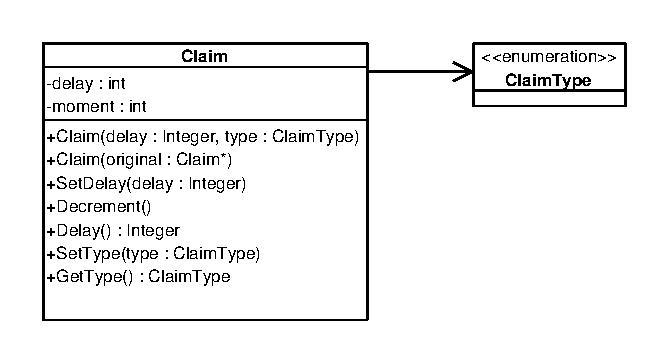
\includegraphics[scale=1]{claim_uml.eps}
	\caption{Класс Claim}
	\label{claim_uml}
\end{figure}
[Пояснение к Claim]

Для реализации подхода, базирующимся на постоянном обновлении состоянии заявок, находящихся в модели, предметная область базируется на общем интерфейсе, который реализуют все конкретные элементы рассматриваемых систем массового обслуживания. Его цель заключается в формализации изменения элемента  с каждым дискретным моментом времени в течение моделирования. Поскольку, сам объект системы массового обслуживания реализует данный интерфейс, то возможно использовать ее как входящий поток для другой системы.
\begin{figure}[H]
	\centering
	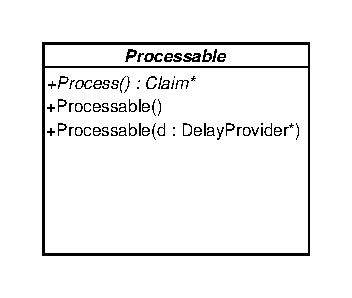
\includegraphics[scale=1]{processable_uml.eps}
	\caption{Общий интерфейс Processable для всех элементов системы массового обслуживания}
	\label{processable_uml}
\end{figure}
[Пояснение к Processable]

Для обеспечения среды, которой будет происходит моделирование, а именно - вестись подсчет прошедшего времени, вызов взаимодействие с реализацией интерфейса Processable и сбор статистики, введен глобальный объект Environment
\begin{figure}[H]
	\centering
	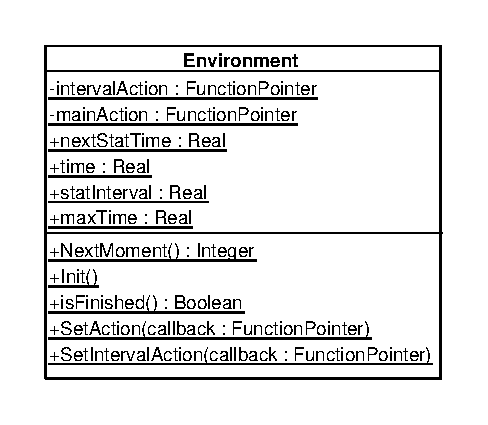
\includegraphics[scale=1]{environment_uml.eps}
	\caption{Глобальный объект Environment}
	\label{environment_uml}
\end{figure}
[Пояснение к Environment]

\subsection{Процесс моделирования} %Имитационное моделирование
\section{Численные эксперименты}
\subsection{Проверка стабильности имитационной модели}
Для начала проведения численного анализа полученных решений необходимо проверить точность работы реализованной имитационной модели. Для проверки, запустим модель несколько раз с одинаковыми параметрами и для полученных результатов вычислим критерий согласия Колмогорова. Критерий согласия Колмогорова (расстояние Колмогорова) предназначен для проверки гипотезы о том, что некое эмпирическое распределение, в данном случае, распределение, построенное в ходе работы имитационной модели, соответствует предполагаемой модели, которая, в данном случае, так же является результатом работы имитационной модели.

Расстояние Колмогорова вычисляется по следующей формуле
\begin{equation*}
	\Delta_{l} = \underset{0 \leq i \leq \infty}{max}\bigg\rvert \sum_{v=0}^{i} (P(v) - P^{l}(v))\bigg\rvert, l = 1,2
\end{equation*}
Для численного анализа в данной работе применяется система компьютерной алгебры Mathcad. В ней были построены графики распределения вероятностей и вычислено расстояния Колмогорова для двух запусков имитационной модели с одинаковыми параметрами системы

\begin{figure}[H]
	\centering
	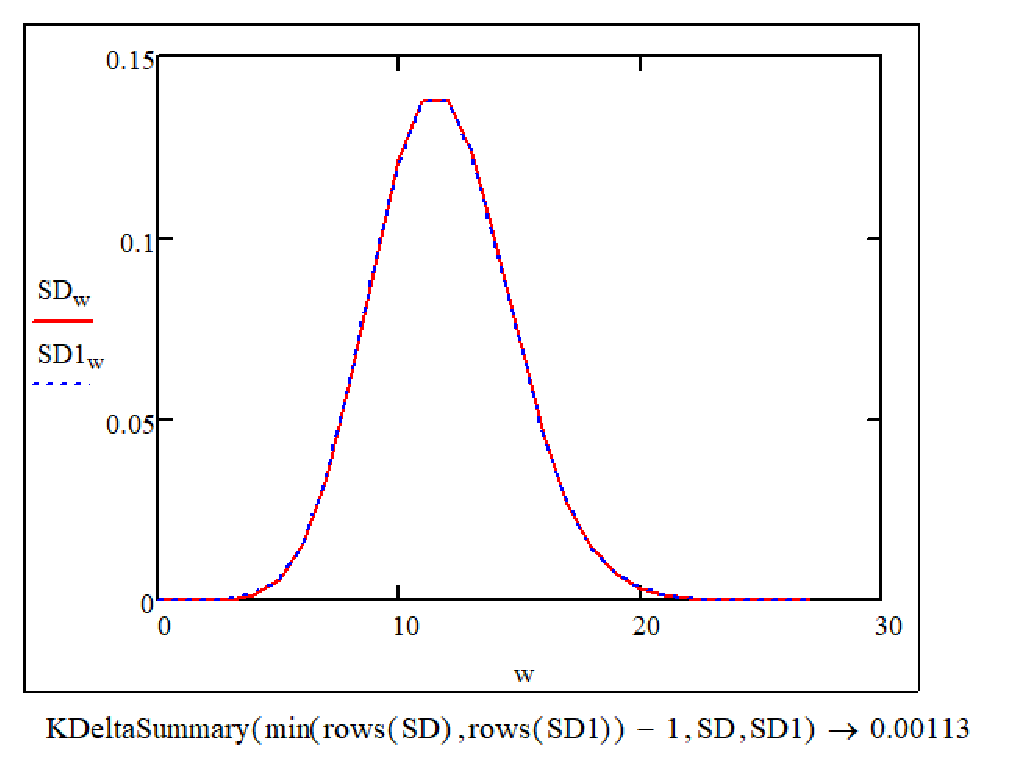
\includegraphics[scale=0.5,width=\textwidth]{mathcad_check_sim.eps}
	\caption{Сравнение двух отдельных запусков имитационной модели с простейшим входящим потоком}
	\label{experiments_kol_dist_sim}
\end{figure} 

На рисунке \ref{experiments_kol_dist_sim} представлено сравнение двух запусков имитационной модели с параметрами системы: $\lambda = 1, \alpha = 0.5, \sigma = 0.4, \mu_{1} = 6, \mu_{2}, t = 10 $. Запуски модели дали практически одинаковые результаты. Вычисленное расстояние Колмогорова составило  0.000596 для суммарного распределения и 0.0016632 для двумерного распределения. Графики плотности распределения вероятностей полностью накладываются друг на друга.

\begin{figure}[H]
	\centering
	\includegraphics[scale=0.5,width=\textwidth]{mathcad_check_sim2.eps}
	\caption{Сравнение двух отдельных запусков имитационной модели с MMPP--потоком}
	\label{experiments_kol_dist_sim2}
\end{figure} 

Данный эксперимент был проведен и для системы с входящим MMPP--потоком. Были заданы следующие параметры: $\alpha = 0.5, \sigma = 0.4, \mu_{1} = 6, \mu_{2}, t = 10 $,
\begin{equation*}
	\boldsymbol{Q}=\begin{bmatrix}
		-0.3 &  0.1 &  0.1\\
		0.2 & -0.5 &  0.3\\
		0.3 &  0.3 &  -0.6
	\end{bmatrix}
\end{equation*}

\begin{equation*}
	\boldsymbol{\Lambda}=\begin{bmatrix}
		1 &	0 & 0\\
		0 &	0.6 & 0\\
		0 &	0 & 0.7\\
	\end{bmatrix}.
\end{equation*}
Результаты эксперимента представлены на рисунке \ref{experiments_kol_dist_sim2}. Для суммарного распределения расстояние Колмогорова составило 0.00059, для двумерного --- 0.001258. Графики плотности распределений также полностью накладываются друг на друга.

Исходя из вышеописанных экспериментов, можно сделать вывод, что реализованная имитационная модель дает стабильные результаты, что подтверждают вычисленные значения расстояния Колмогорова для обоих видов распределений, следовательно, модель можно использовать для анализа полученных решений и оценки их применимости.
\subsection{Сравнение распределений вероятностей с эмпирическим распределением}
Теперь, когда стабильность имитационной модели подтверждена экспериментально, сравним результаты ее работы с полученным асимптотическим приближением функции распределения вероятностей числа обслуженных заявок для систем, рассмотренных в разделах \ref{section_simple_summary}, \ref{section_simple_twodim} и \ref{section_map_twodim} при разной интенсивности возврата заявок с орбиты. Значение этого параметра влияет на точность при сравнении, так как решение систем было получено при асимптотическом условии большой задержки заявок на орбите.

Для того, чтобы проиллюстрировать влияние задержки заявок на орбите на получаемый результат, зададим исходные параметры:
\begin{equation} \label{simple_summary_input_params}
	\lambda = 2,
	\alpha = 0.9,
	\mu_{1} = 3.5,
	\mu_{2} = 2.1, 
	t = 15
\end{equation}
Теперь, рассчитаем распределения вероятностей числа обслуженных заявок по формуле \eqref{distr_simple_summary} и запустим имитационную модель, варьируя интенсивность возращения заявок с орбиты $\sigma$

\begin{table}[h!] 
	\centering
	\caption{Расстояние Колмогорова при различных значениях параметра $\sigma$}
	\label{table_simple_summary}
	\begin{tabular}{ | c | c | c | c | c | c | c | c |}
		\hline
		$\sigma$ & 1 & 0.6 & 0.4 & 0.2 & 0.1 & 0.05 & 0.01 \\ 
		\hline
		$\Delta_S$ & 0.0148 & 0.0112 & 0.0096 & 0.0062 & 0.0044 & 0.0023 & 0.0019\\
		\hline
		$\Delta_{TD}$ & 0.02619 & 0.0205 & 0.0153 & 0.0088 & 0.0056 & 0.0025 & 0.0019\\
		\hline
	\end{tabular}
\end{table}

Как видно в таблице \ref{table_simple_summary}, при сравнении работы имитационной модели и асимптотических результатов расстояние Колмогорова тем меньше, чем меньше интенсивность возврата заявок с орбиты. Однако, даже при больших значениях $\sigma$, таких как 1 и 0.6, мы получаем результаты, где расстояние Колмогорова составляет не больше двух сотых. В нижней строчке таблицы \ref{table_simple_summary} представлены расчеты для двумерного распределения вероятности числа обслуженных заявок. Можно видеть, что в случае двумерного распределения расстояние Колмогорова значительно больше при больших значениях $\sigma$, однако оно сходится к такому же значению при $\sigma = 0.01$, что и в случае одномерного распределения.

Чтобы проверить, наблюдается ли подобная тенденция при большей загруженности системы, установим в ранее описанных параметрах \eqref{simple_summary_input_params} $\lambda = 2.7$. Тогда получим следующий результат

\begin{table}[h!] 
	\centering
	\caption{Расстояние Колмогорова при различных значениях параметра $\sigma$ при повышенной интенсивности прихода заявок}
	\label{table_simple_summary_high_lambda}
	\begin{tabular}{ | c | c | c | c | c | c | c | c |}
		\hline
		$\sigma$ & 1 & 0.6 & 0.4 & 0.2 & 0.1 & 0.05 & 0.01 \\ 
		\hline
		$\Delta_S$ & 0.0044 & 0.0039 & 0.0028 & 0.003 & 0.0025 & 0.0013 & 0.0016\\
		\hline
		$\Delta_{TD}$ & 0.0104 & 0.0074 & 0.0044 & 0.0034 & 0.0021 & 0.0017 & 0.0011\\
		\hline
	\end{tabular}
\end{table}

Как видно в таблице \ref{table_simple_summary_high_lambda}  при повышенной загруженности системы также наблюдается тенденция к уменьшению расстоянию Колмогорова, однако, асимптотические результаты оказываются значительно точнее.

Поскольку интенсивность вызова прибором заявок также непосредственно влияет на количество заявок на орбите, проведем расчеты с параметрами \eqref{simple_summary_input_params}, установив $\alpha = 1.6$

\begin{table}[h!] 
	\centering
	\caption{Расстояние Колмогорова при различных значениях параметра $\sigma$ при повышенной интенсивности вызова заявок}
	\label{table_simple_summary_high_alpha}
	\begin{tabular}{ | c | c | c | c | c | c | c | c |}
		\hline
		$\sigma$ & 1 & 0.6 & 0.4 & 0.2 & 0.1 & 0.05 & 0.01 \\ 
		\hline
		$\Delta_S$ & 0.0062 & 0.0051 & 0.0054 & 0.0053 & 0.0023 & 0.0013 & 0.002\\
		\hline
		$\Delta_{TD}$ & 0.015 & 0.0111 & 0.0096 & 0.0069 & 0.0029 & 0.0015 & 0.0011\\
		\hline
	\end{tabular}
\end{table}

Из расчетов в таблице \ref{table_simple_summary_high_alpha} видно, что также при увеличении задержки заявок на орбите, асимптотические результаты становятся точнее, однако повышение интенсивности вызова прибором заявок делает расчеты менее закономерными.

Для проведения данного эксперимента с RQ--системой, где в качестве источника заявок выступает MMPP--потоком, зададим следующие параметры:
\begin{equation*} \label{map_summary_input_params}
	\alpha = 0.6,
	\mu_{1} = 2,
	\mu_{2} = 1.5, 
	t = 15,
\end{equation*}
 \begin{equation*}
 	\boldsymbol{Q}=\begin{bmatrix}
 		-0.5 &  0.2 &  0.3\\
 		0.15 & -0.2 &  0.05\\
 		0.3 &  0.4 &  -0.7
 	\end{bmatrix},
 \end{equation*}
 
 \begin{equation*}
 	\boldsymbol{\Lambda}=\begin{bmatrix}
 		1 &	0 & 0\\
 		0 &	0.6 & 0\\
 		0 &	0 & 0.7\\
 	\end{bmatrix}.
 \end{equation*}
Были получены следующие результаты
\begin{table}[h!] 
	\centering
	\caption{Расстояние Колмогорова при различных значениях параметра $\sigma$ при моделировании MMPP-потока}
	\label{table_map_summary}
	\begin{tabular}{ | c | c | c | c | c | c | c | c |}
		\hline
		$\sigma$ & 1 & 0.6 & 0.4 & 0.2 & 0.1 & 0.05 & 0.01 \\ 
		\hline
		$\Delta_S$ & 0.045 & 0.0407 & 0.0359 & 0.0282 & 0.023 & 0.018 & 0.0163\\
		\hline
		$\Delta_{TD}$ & 0.0493 & 0.0415 & 0.0348 & 0.0236 & 0.0154 & 0.009 & 0.0028\\
		\hline
	\end{tabular}
\end{table}

Ввиду того, что MMPP--поток труднее поддается моделированию, расстояние Колмогорова для расчетов с ним в среднем больше, однако при маленьких значениях $\sigma$ точность значительно увеличивается. Также, на таблице \ref{table_map_summary} можно заметить, что при меньших $\sigma$ для двумерного распределения асимптотические результаты оказываются точнее.

Повысим загруженность системы, задав новую матрицу интенсивностей с более высокими значениями диагональных элементов 
 \begin{equation*}
	\boldsymbol{\Lambda}=\begin{bmatrix}
		1.2 &	0 & 0\\
		0 &	0.9 & 0\\
		0 &	0 & 1.5\\
	\end{bmatrix}.
\end{equation*}
Проведем эксперимент с новыми параметрами и получим
\begin{table}[h!] 
	\centering
	\caption{Расстояние Колмогорова при различных значениях параметра $\sigma$ при повышенной интенсивности вызова заявок}
	\label{table_map_summary_high_lambda}
	\begin{tabular}{ | c | c | c | c | c | c | c | c |}
		\hline
		$\sigma$ & 1 & 0.6 & 0.4 & 0.2 & 0.1 & 0.05 & 0.01 \\ 
		\hline
		$\Delta_S$ & 0.0285 & 0.0244 & 0.0205 & 0.0145 & 0.0108 & 0.0077 & 0.0082\\
		\hline
		$\Delta_{TD}$ & 0.0478 & 0.039 & 0.0312 & 0.0191 & 0.0105 & 0.0055 & 0.002\\
		\hline
	\end{tabular}
\end{table}
На основании проведенных экспериментов можно сделать вывод, что тенденция к увеличению точности асимптотических результатов всегда наблюдается при уменьшении значения $\sigma$. Также, повышение загруженности системы заявками входящего потока, как это видно в таблицах \ref{table_simple_summary},\ref{table_simple_summary_high_lambda} и \ref{table_map_summary},\ref{table_map_summary_high_lambda}, положительно влияют на точность асимптотических результатов, в то время как увеличение интенсивности вызова заявок прибором делают результаты менее закономерными.

\subsection{Анализ корреляции выходящих процессов}
Как было упомянуто ранее, основной целью исследования является корреляции компонентов двумерного выходящего потока рассматриваемого узла обработки запросов. В данном разделе проводится анализ коэффициента корреляции выходящих процессов %Численные эксперименты
\titleformat{\section}[block]
{\normalsize\bfseries\centering}
{\thesection}
{1em}{}
\section*{\centering\normalsize ЗАКЛЮЧЕНИЕ}
\addcontentsline{toc}{section}{Заключение}
В рамках данной работы был рассмотрен ряд Марковских систем массового обслуживания с повторными вызовами и вызываемыми заявками, имеющих в качестве источника заявок простейший и MMPP--потоки. Согласно указанной цели исследования был выполнен ряд задач.

Были построены математические модели функционирования рассматриваемых узлов обработки запросов. В зависимости от типа системы, описывающий ее Марковский процесс имеет разную размерность. Так, для системы с одномерным выходящим потоком и простейшим входящим он будет трехмерным --- $\{k(t),i(t),m(t)\}$, при построении модели с разными типами заявок был добавлен процесс $m_{2}(t)$, а для системы с входящим потоком MMPP--потоком был добавлен процесс $n(t)$, описывающий состояние управляющей цепи MMPP. На основе Марковских процессов были составлены системы уравнений Колмогорова. Для нахождения характеристик выходящего потока был осуществлен переход к характеристическим функциям и применен метод асимптотического анализа в предельном условии большой задержки заявок на орбите. В результате были получены формулы (\ref{approximation_summary},\ref{approximation_twodim},\ref{approximation_twodim_map}) для вычисления асимптотического приближения характеристической функции числа заявок, окончивших обслуживание в системе к моменту времени $t$.

Для вычисления значений распределения вероятностей числа обслуженных заявок были получены формулы (\ref{distr_simple_summary},\ref{distr_simple_twodim},\ref{distr_map_twodim}), в которых используется преобразование подобия матриц для вычисления матричной экспоненты и обратное преобразование Фурье, позволяющее перейти от характеристической функции к явному виду распределения вероятностей. Помимо этого, в разделе \ref{corr_section} были приведены выкладки для вычисления коэффициента корреляции компонентов двумерного распределения при помощи полученных асимптотических приближений характеристической функции числа обслуженных заявок. Применение указанных формул позволило проводить анализ решений в системе компьютерной алгебры Mathcad и при заданных параметрах системы получать численные характеристики работы системы.

Для оценки применимости полученных асимптотических результатов был разработан и реализован программный продукт, позволяющий проводить имитационное моделирование рассматриваемых систем. В первую очередь, были выделены сущности, принадлежащие к предметной области работы. Далее, была построена объектная модель программы, позволяющая расширять набор используемых элементов теории массового обслуживания при помощи общего для них интерфейса, формализующего изменение состояния элемента при наступлении очередного события в модели. Процесс моделирования, заключающийся в регистрации моментов наступления событий, позволил проводить моделирование итеративно и регистрировать необходимые для анализа характеристики работы системы. Реализация программы представляет собой две составных части - библиотеку, реализованная с учетом построенной объектной модели и оболочку для ее использования с графическим пользовательским интерфейсом. Раздельная реализация дает возможность легко добавлять новый функционал к имеющемуся.  

Процесс работы с программой предусматривает два подхода. В первом случае, по умолчанию, моделирование производится в реальном времени с настраиваемым интервалом таймера, который отсчитывает проведение следующей итерации моделирования. Данный подход дает возможность пользователю получать результаты моделирования и проводить их предварительный анализ с помощью встроенных графических средств, таких как трехмерное представление распределения вероятностей с возможностью масштабирования и выделения необходимой области с отсечением. Второй способ позволяет быстро получить результаты моделирования для последующего анализа с помощью других программных средств, для чего реализована функция экспорта данных распределения вероятностей в текстовый формат. 

Имитационная модель была протестирована на стабильность получаемых результатов при помощи расстояния Колмогорова. В ходе эксперимента его значение не превышало 0.002, что говорит о высокой стабильности моделирования.

Из-за асимптотической природы полученных результатов встает вопрос об их применимости на практике в реальных системах, соответствующих рассматриваемых моделям. Для ее оценки была применена указанная имитационная модель и расстояние Колмогорова, показывающие, насколько соответствует эмпирическое распределение вероятностей предложенной модели. Расчеты показали, что при увеличении задержки заявок на орбите аналитические формулы дают более точное распределение вероятностей числа обслуженных заявок. Такой результат является закономерным ввиду того, что аналитические решения были получены при соответствующем асимптотическом условии, однако, даже при меньшей задержке заявок на орбите расчеты оказываются достаточно точными, чтобы их можно было применять на практике. Внимания требует так же распределение вероятностей, получаемое при большей загруженности системы. В таких условиях расчеты становятся еще более точными. В ходе проведенных численных экспериментов значение расстояния Колмогорова не превышало 0.066 --- данный результат был получен при увеличенной загрузке системы с MMPP--потоком при интенсивности возврата заявок с орбиты равной 10.

Для рассматриваемых систем был проведен численный анализ корреляции выходящих процессов, в ходе которого были выявлены некоторые закономерности изменения их корреляции при различных параметрах системы. В частности, при варьировании параметров для разных типов заявок коэффициент корреляции всегда меньше нуля и тем меньше, чем больше интенсивность поступления заявок, входящих либо вызываемых, в систему; в то время как при изменении параметров системы для одного типа заявок коэффициент корреляции принимает как положительные, так и отрицательные значения. Также были найдены параметры системы, при которых компоненты выходящего потока становятся независимыми. Эти результаты крайне важны для понимая функционирования выходящих процессов системы, однако для интерпретации этого открытия требуется дальнейшее исследование.

В конечном итоге, проведенное исследование позволяет применять полученные в ходе него аналитические решения и результаты численного анализа  для изучения функционирования и отладки реальных систем массового обслуживания \cite{deering1991icmp,nutt1982performance} с высокой точностью. Крайне важным и трудно исследуемым аспектом функционирования таких систем является выходящих поток обслуженных требований, поскольку он представляет собой характеристику работы системы в совокупности, а она, в свою очередь, зависит от других процессов, происходящих в рамках системы. Помимо этого, исследование выходящего потока требований и его характеристик является необходимым при построении телекоммуникационных сетей, поскольку обслуженные требования одного узла является входящими для другого, что для сетей значительного размера представляет собой еще более важный аспект проектирования.

Результаты проведенного исследования были представлены в качестве докладов и обсуждались на пяти международных конференциях:
\begin{itemize}
\item XIX Международная конференции по информационным технологиям и математическому моделированию имени А.Ф. Терпугова (ITMM) (май 2020, Томск);
\item VIII Международная молодежная научная конференция «Математическое и программное обеспечение информационных, технических и экономических систем» (май 2021, Томск);
\item VII Международная конференция «Математика, её приложения и математическое образование» (МПМО) (сентябрь 2020, Улан-Удэ);
\item V Международная конференции по стохастическим методам (ноябрь 2020, Москва);
\item VII Международная молодеждная научная конференция \textquote{Математическое и программное обеспечение информационных, технических и экономических систем} (май 2020, Томск).
\end{itemize}
Материалы, представленные в работе были опубликованы в трех сборниках материалов конференций \cite{itmm_2021,icsm,mpmo} и одной статье, индексируемой в Scopus \cite{blaginin2020two}. Также, для основного алгоритма имитационной модели было получено свидетельство о регистрации программы для ЭВМ \cite{evm}.
 \clearpage %Заключение
\bibliographystyle{ugost2008mod}
\addcontentsline{toc}{section}{Список использованной литературы}
\bibliography{refs.bib}\nocite{*}
\clearpage
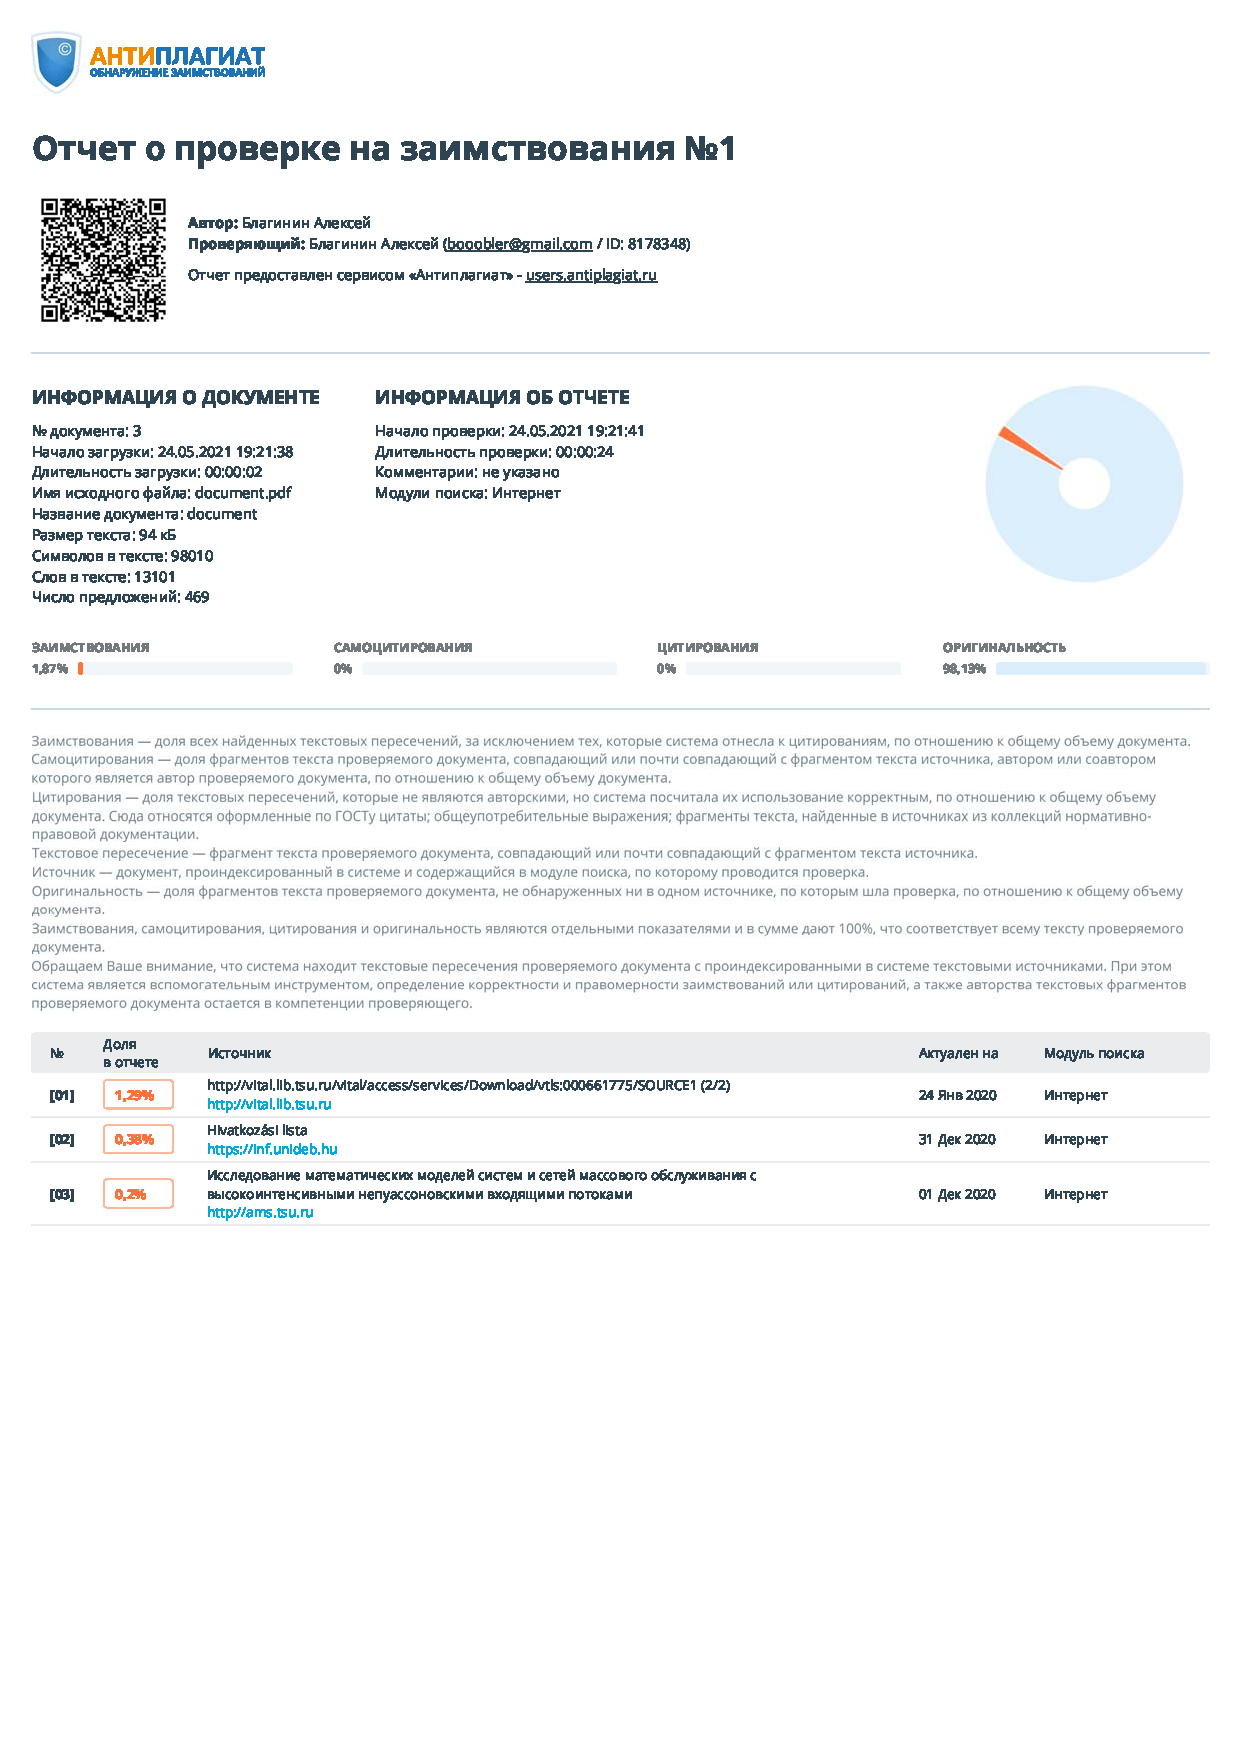
\includepdf[pagetemplate=1,scale=0.83,offset=0.75cm 0]{antiplagiat}
\end{document}